% Options for packages loaded elsewhere
\PassOptionsToPackage{unicode}{hyperref}
\PassOptionsToPackage{hyphens}{url}
%
\documentclass[
]{article}
\usepackage{amsmath,amssymb}
\usepackage{lmodern}
\usepackage{iftex}
\ifPDFTeX
  \usepackage[T1]{fontenc}
  \usepackage[utf8]{inputenc}
  \usepackage{textcomp} % provide euro and other symbols
\else % if luatex or xetex
  \usepackage{unicode-math}
  \defaultfontfeatures{Scale=MatchLowercase}
  \defaultfontfeatures[\rmfamily]{Ligatures=TeX,Scale=1}
\fi
% Use upquote if available, for straight quotes in verbatim environments
\IfFileExists{upquote.sty}{\usepackage{upquote}}{}
\IfFileExists{microtype.sty}{% use microtype if available
  \usepackage[]{microtype}
  \UseMicrotypeSet[protrusion]{basicmath} % disable protrusion for tt fonts
}{}
\makeatletter
\@ifundefined{KOMAClassName}{% if non-KOMA class
  \IfFileExists{parskip.sty}{%
    \usepackage{parskip}
  }{% else
    \setlength{\parindent}{0pt}
    \setlength{\parskip}{6pt plus 2pt minus 1pt}}
}{% if KOMA class
  \KOMAoptions{parskip=half}}
\makeatother
\usepackage{xcolor}
\IfFileExists{xurl.sty}{\usepackage{xurl}}{} % add URL line breaks if available
\IfFileExists{bookmark.sty}{\usepackage{bookmark}}{\usepackage{hyperref}}
\hypersetup{
  hidelinks,
  pdfcreator={LaTeX via pandoc}}
\urlstyle{same} % disable monospaced font for URLs
\usepackage{graphicx}
\makeatletter
\def\maxwidth{\ifdim\Gin@nat@width>\linewidth\linewidth\else\Gin@nat@width\fi}
\def\maxheight{\ifdim\Gin@nat@height>\textheight\textheight\else\Gin@nat@height\fi}
\makeatother
% Scale images if necessary, so that they will not overflow the page
% margins by default, and it is still possible to overwrite the defaults
% using explicit options in \includegraphics[width, height, ...]{}
\setkeys{Gin}{width=\maxwidth,height=\maxheight,keepaspectratio}
% Set default figure placement to htbp
\makeatletter
\def\fps@figure{htbp}
\makeatother
\setlength{\emergencystretch}{3em} % prevent overfull lines
\providecommand{\tightlist}{%
  \setlength{\itemsep}{0pt}\setlength{\parskip}{0pt}}
\setcounter{secnumdepth}{-\maxdimen} % remove section numbering
\ifLuaTeX
  \usepackage{selnolig}  % disable illegal ligatures
\fi

\author{}
\date{}

\begin{document}

\hypertarget{header-n320}{%
\section{Experimental report for the 2021 COM1005 Assignment: The
Rambler's Problem}\label{header-n320}}

\begin{itemize}
\item
  GitHub:
  \href{https://github.com/JiaaoWang04/COM1005_Assignment_Report.git}{link}
\item
  Date: 2021/05/24
\end{itemize}

\hypertarget{header-n327}{%
\subsection{Description of my branch-and-bound
implementation}\label{header-n327}}

Maintain two lists

\begin{itemize}
\item
  \emph{open} is used to store the nodes to be processed
\item
  \emph{closed} is used to store the nodes that have been processed
\end{itemize}

When the \emph{open} list is not empty, perform the following operations

\begin{enumerate}
\def\labelenumi{\arabic{enumi}.}
\item
  Each time the node \(n\) with the smallest \(n.GC\) is selected from
  the \emph{open} list, and then the node \(n\) is removed from the
  \emph{open} list.
\item
  If node \(n\) is the target node, then node \(n\) and its
  corresponding path are the optimal path
\item
  If the node \(n\) is not the target node

  \begin{enumerate}
  \def\labelenumii{\arabic{enumii}.}
  \item
    Generate \(k\) successor nodes \(s_1, s_2, ..., s_k\) and set the
    corresponding \emph{Local cost} \(s_i.LC\) and \emph{Global cost}
    \(s_i.GC\) (\(s_i.GC = s_i. LC + n.GC\)). In this experiment, the
    calculation of \(s_i.LC\) uses the \emph{Rambler's} algorithm.
  \item
    Traverse the \emph{open} list, whether there is a node \(n_i\) and
    \(s_i\) that represent the same coordinate \((y, x)\), if it exists
    and \(s_i.GC <n_i.GC\), use the state of \(s_i\) Replace the status
    of \(n_i\)
  \item
    Add \(s_{1...4}\) to the \emph{open} list
  \item
    Add node \(n\) to the \emph{closed} list
  \item
    Repeat step 1
  \end{enumerate}
\end{enumerate}

\hypertarget{header-n353}{%
\subsection{Description of my A* implementation}\label{header-n353}}

Maintain two lists

-\emph{open} is used to store the nodes to be processed\\
-\emph{closed} is used to store the nodes that have been processed

When the \emph{open} list is not empty, perform the following operations

\begin{enumerate}
\def\labelenumi{\arabic{enumi}.}
\item
  Each time the node \(n\) with the smallest \(n.RemRC\) is selected
  from the \emph{open} list, then the node \(n\) is removed from the
  \emph{open} list.
\item
  If node \(n\) is the target node, then node \(n\) and its
  corresponding path are the optimal path
\item
  If the node \(n\) is not the target node

  \begin{enumerate}
  \def\labelenumii{\arabic{enumii}.}
  \item
    Generate \(k\) successor nodes \(s_1, s_2, ..., s_k\) and set the
    corresponding \emph{Estimated remained cost} \(s_i.RemRC\)
    (\(s_i.RemRC = H(s_i)\)), *Local cost * \(s_i.LC\), \emph{Global
    cost} \(s_i.GC\) (\(s_i.GC = s_i.LC + n.GC\)).
  \item
    Traverse the \emph{open} list, whether there is a node \(n_i\) and
    \(s_i\) that represent the same coordinate \((y, x)\), if it exists
    and \(s_i.GC <n_i.GC\), use the state of \(s_i\) Replace the status
    of \(n_i\)
  \item
    Add \(s_{1...4}\) to the \emph{open} list
  \item
    Add node \(n\) to the \emph{closed} list
  \item
    Repeat step 1
  \end{enumerate}
\end{enumerate}

The realization of the *A\textbackslash** algorithm is the same as the
basic steps of \emph{branch-and-bound}, only a slight change is made
when the node \emph{n} is selected from \emph{open}, according to the
estimated result of the heuristic function \emph{Estimated Remained
Cost}.

\hypertarget{header-n376}{%
\subsection{Assessing the efficiency of my branch-and-bound search
algorithm}\label{header-n376}}

The following are three sets of experiments. The map data used in each
set of experiments comes from the file "diablo.pgm". The software in the
picture is located in the source code "RunRamblersSwing.java". In the
picture, the \textbf{blue square} represents the starting point of the
search, the \textbf{red square} represents the end of the search, the
\textbf{purple line} represents the search path, \textbf{green The box}
means that the state of a node in the \emph{closed list} corresponds to
a certain coordinate on the map.

\begin{itemize}
\item
  Experiment 1

  \begin{itemize}
  \item
    Experiment content: When the path is a complex path, the situation
    of the \emph{closed list} in the path finding process
  \item
    Experimental results:

    \begin{figure}
    \centering
    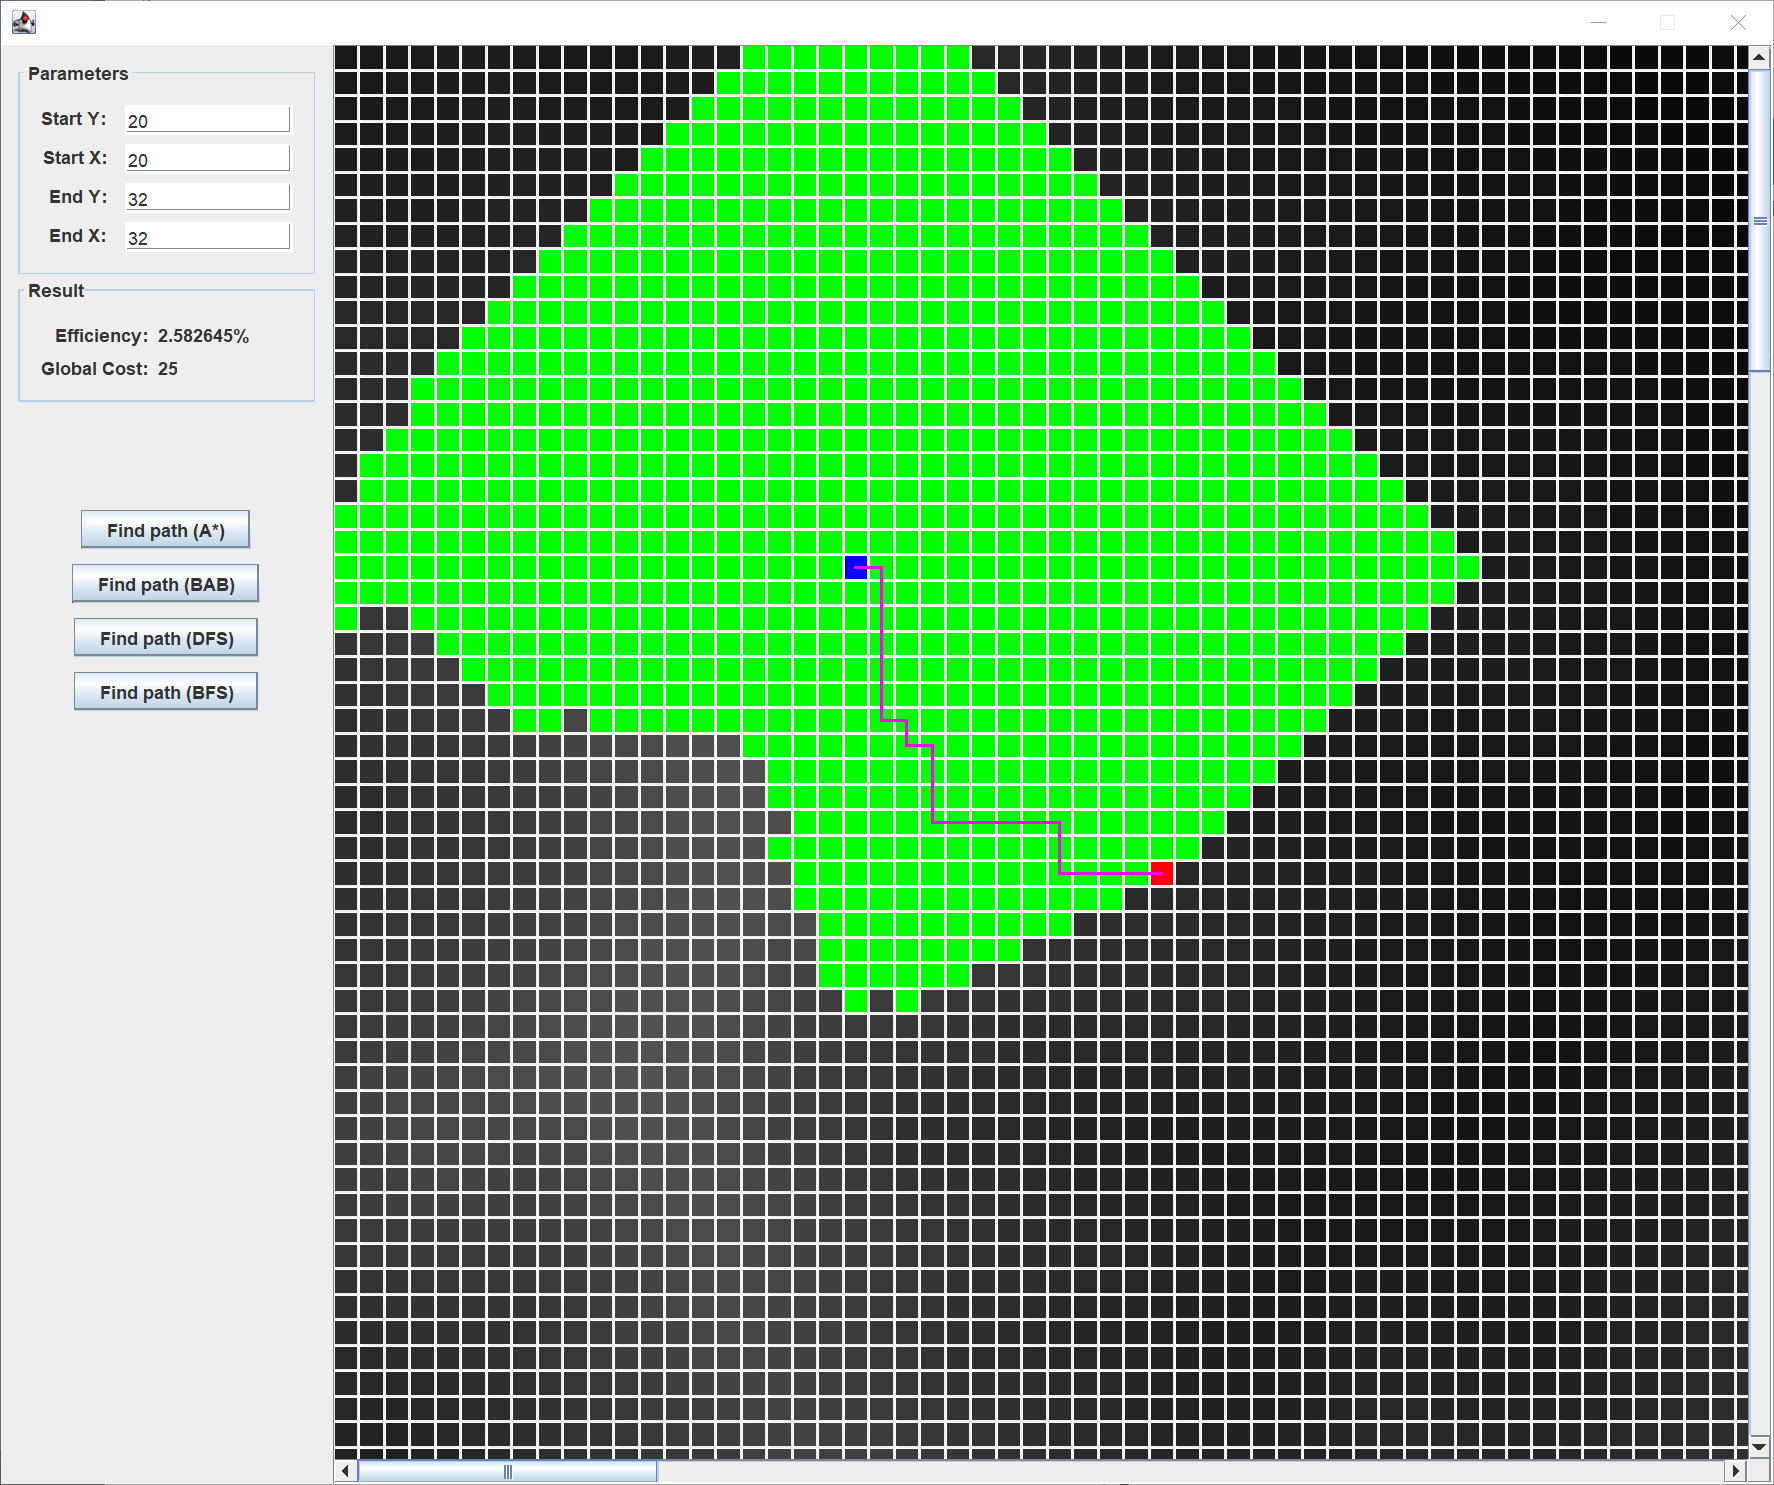
\includegraphics{./images/image-20210523071650111.png}
    \caption{}
    \end{figure}
  \end{itemize}
\item
  Experiment 2

  \begin{itemize}
  \item
    Experiment content: When the path is a straight path, the situation
    of the \emph{closed list} in the path finding process
  \item
    Experimental results:

    \begin{figure}
    \centering
    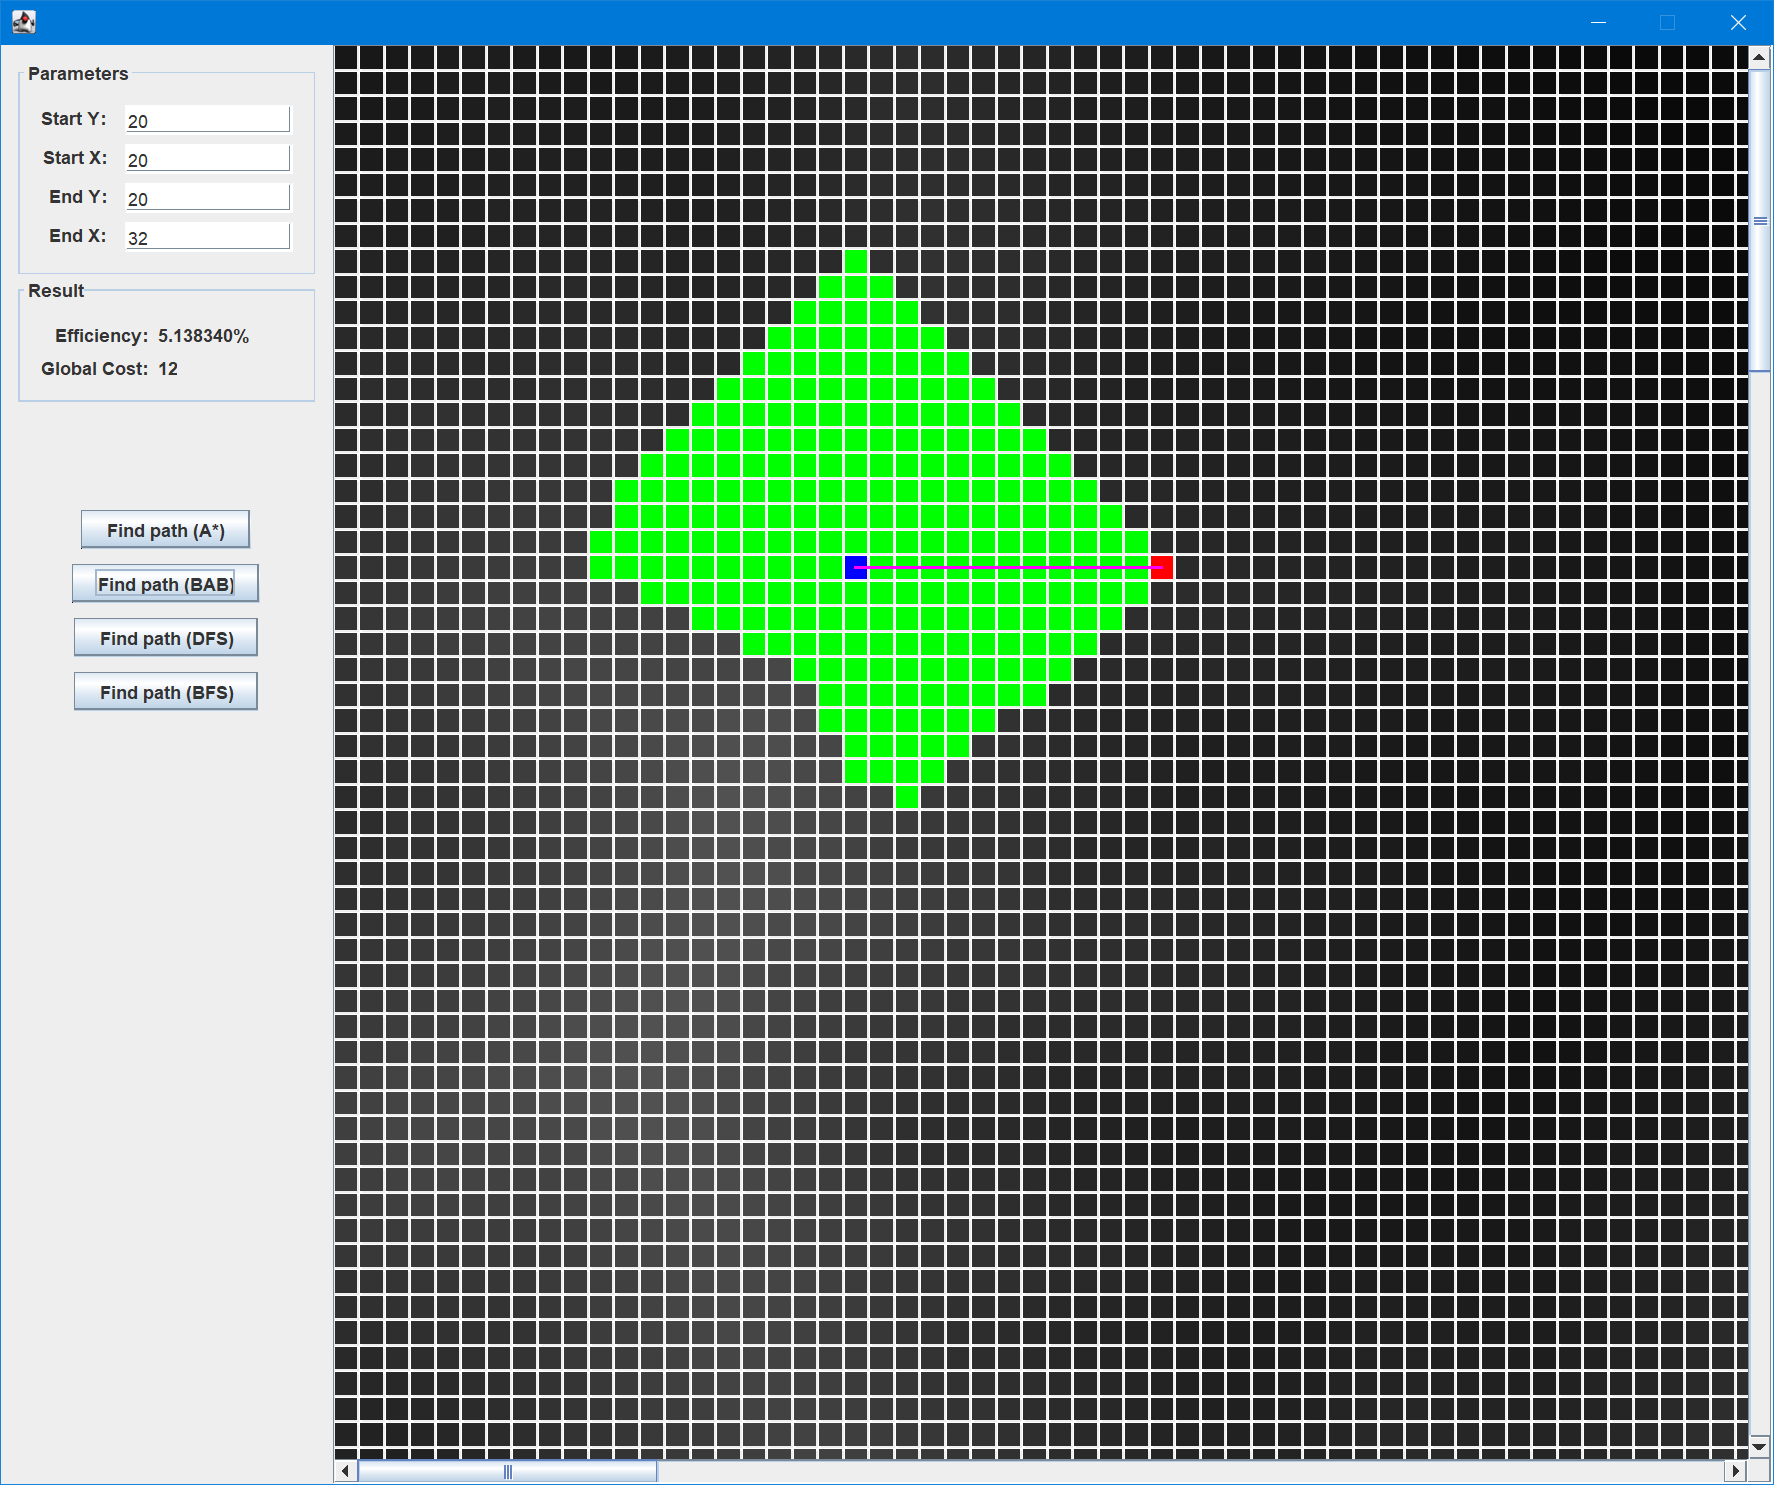
\includegraphics{./images/image-20210523071939104.png}
    \caption{}
    \end{figure}

    \begin{figure}
    \centering
    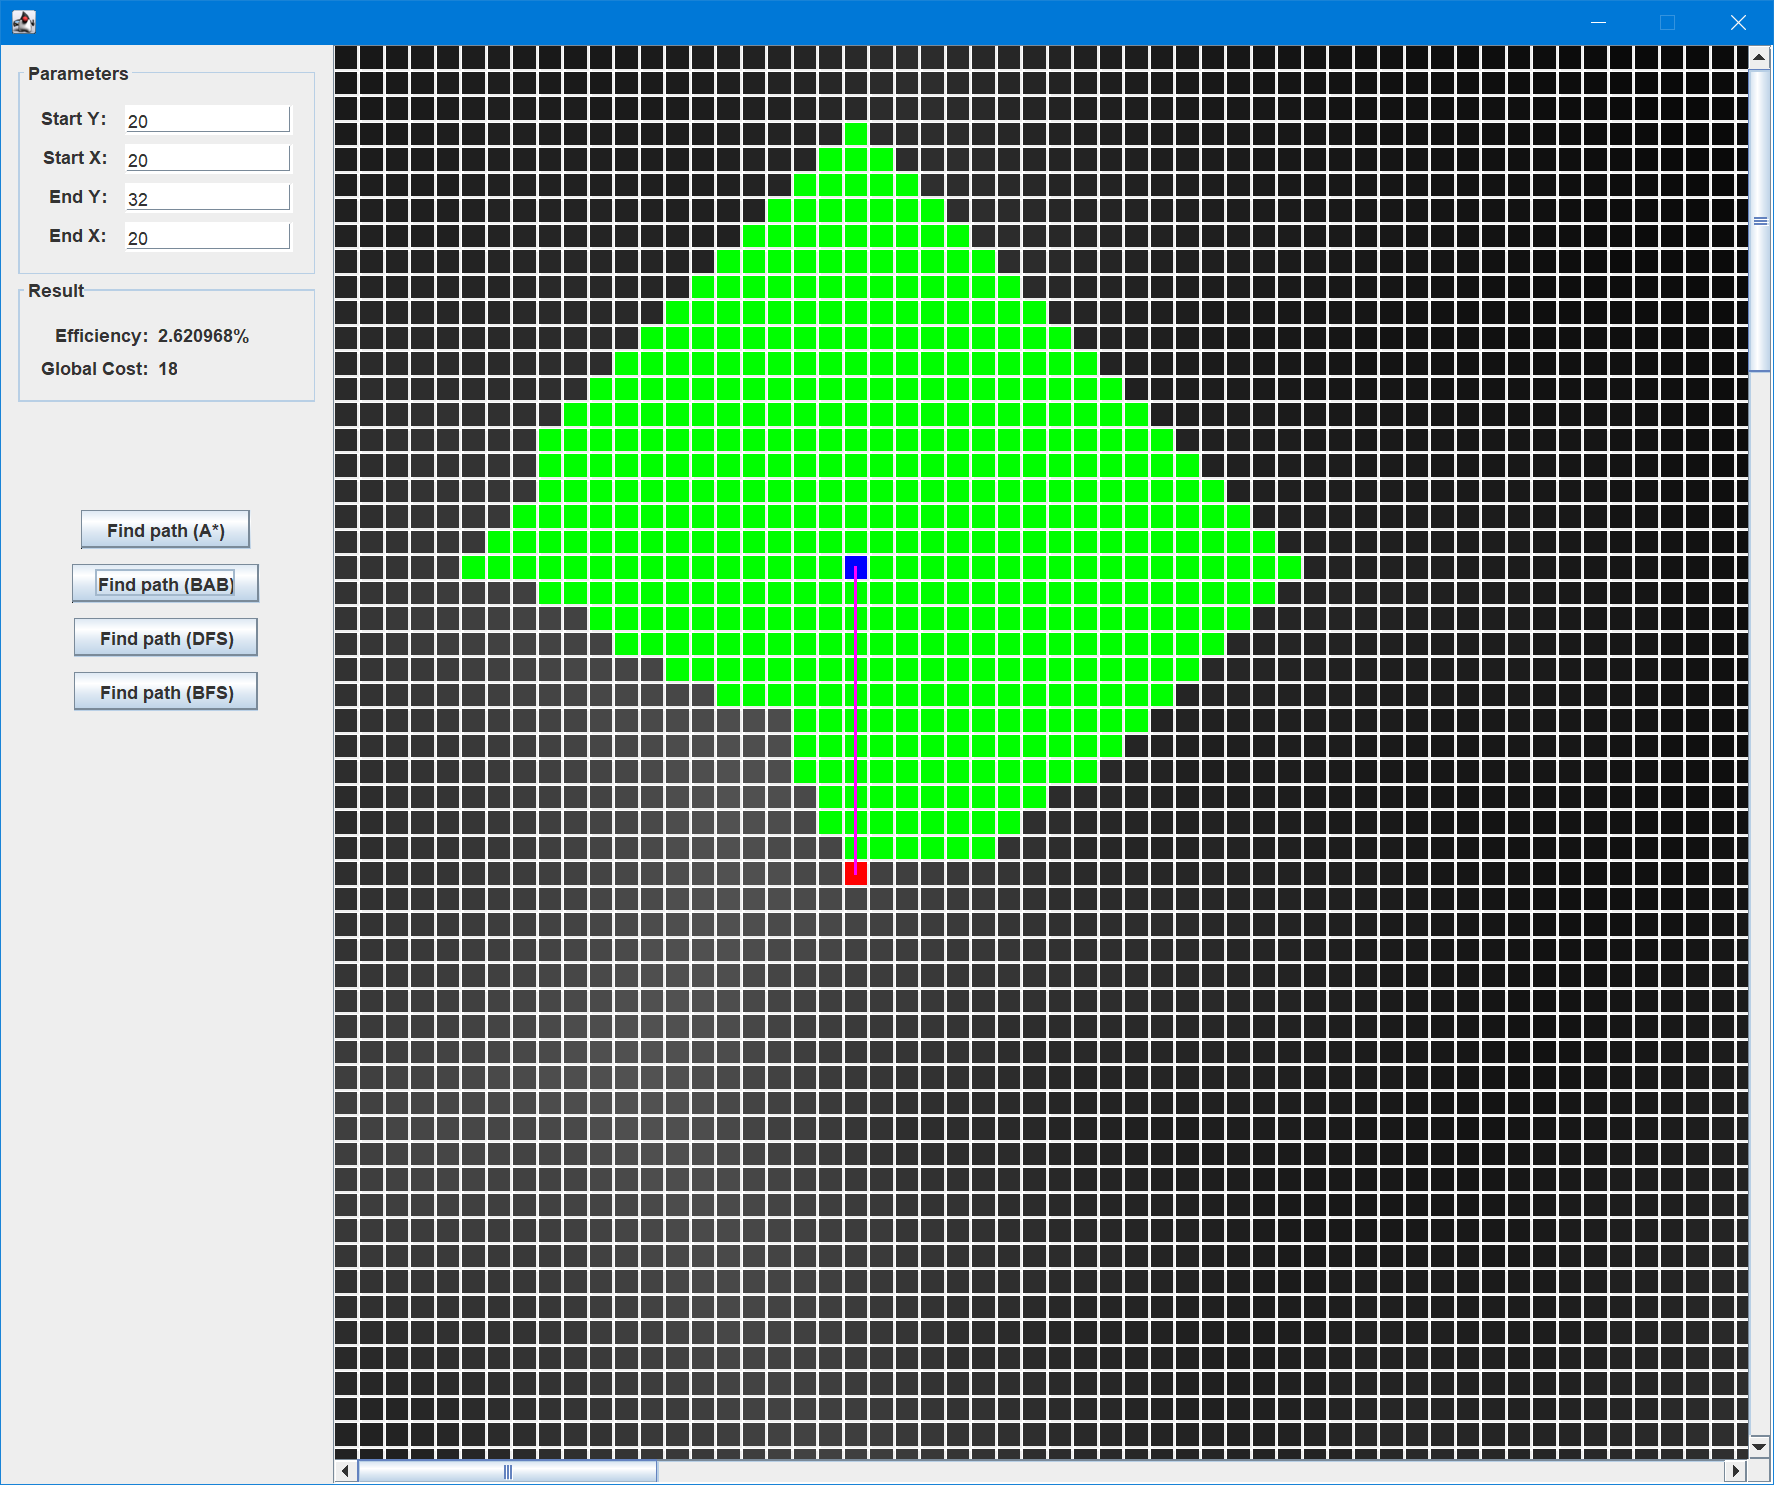
\includegraphics{./images/image-20210523071951327.png}
    \caption{}
    \end{figure}
  \end{itemize}
\item
  Experiment 3

  \begin{itemize}
  \item
    Experiment content: the influence of path length on \emph{closed
    list}
  \item
    Experimental results:

    \begin{figure}
    \centering
    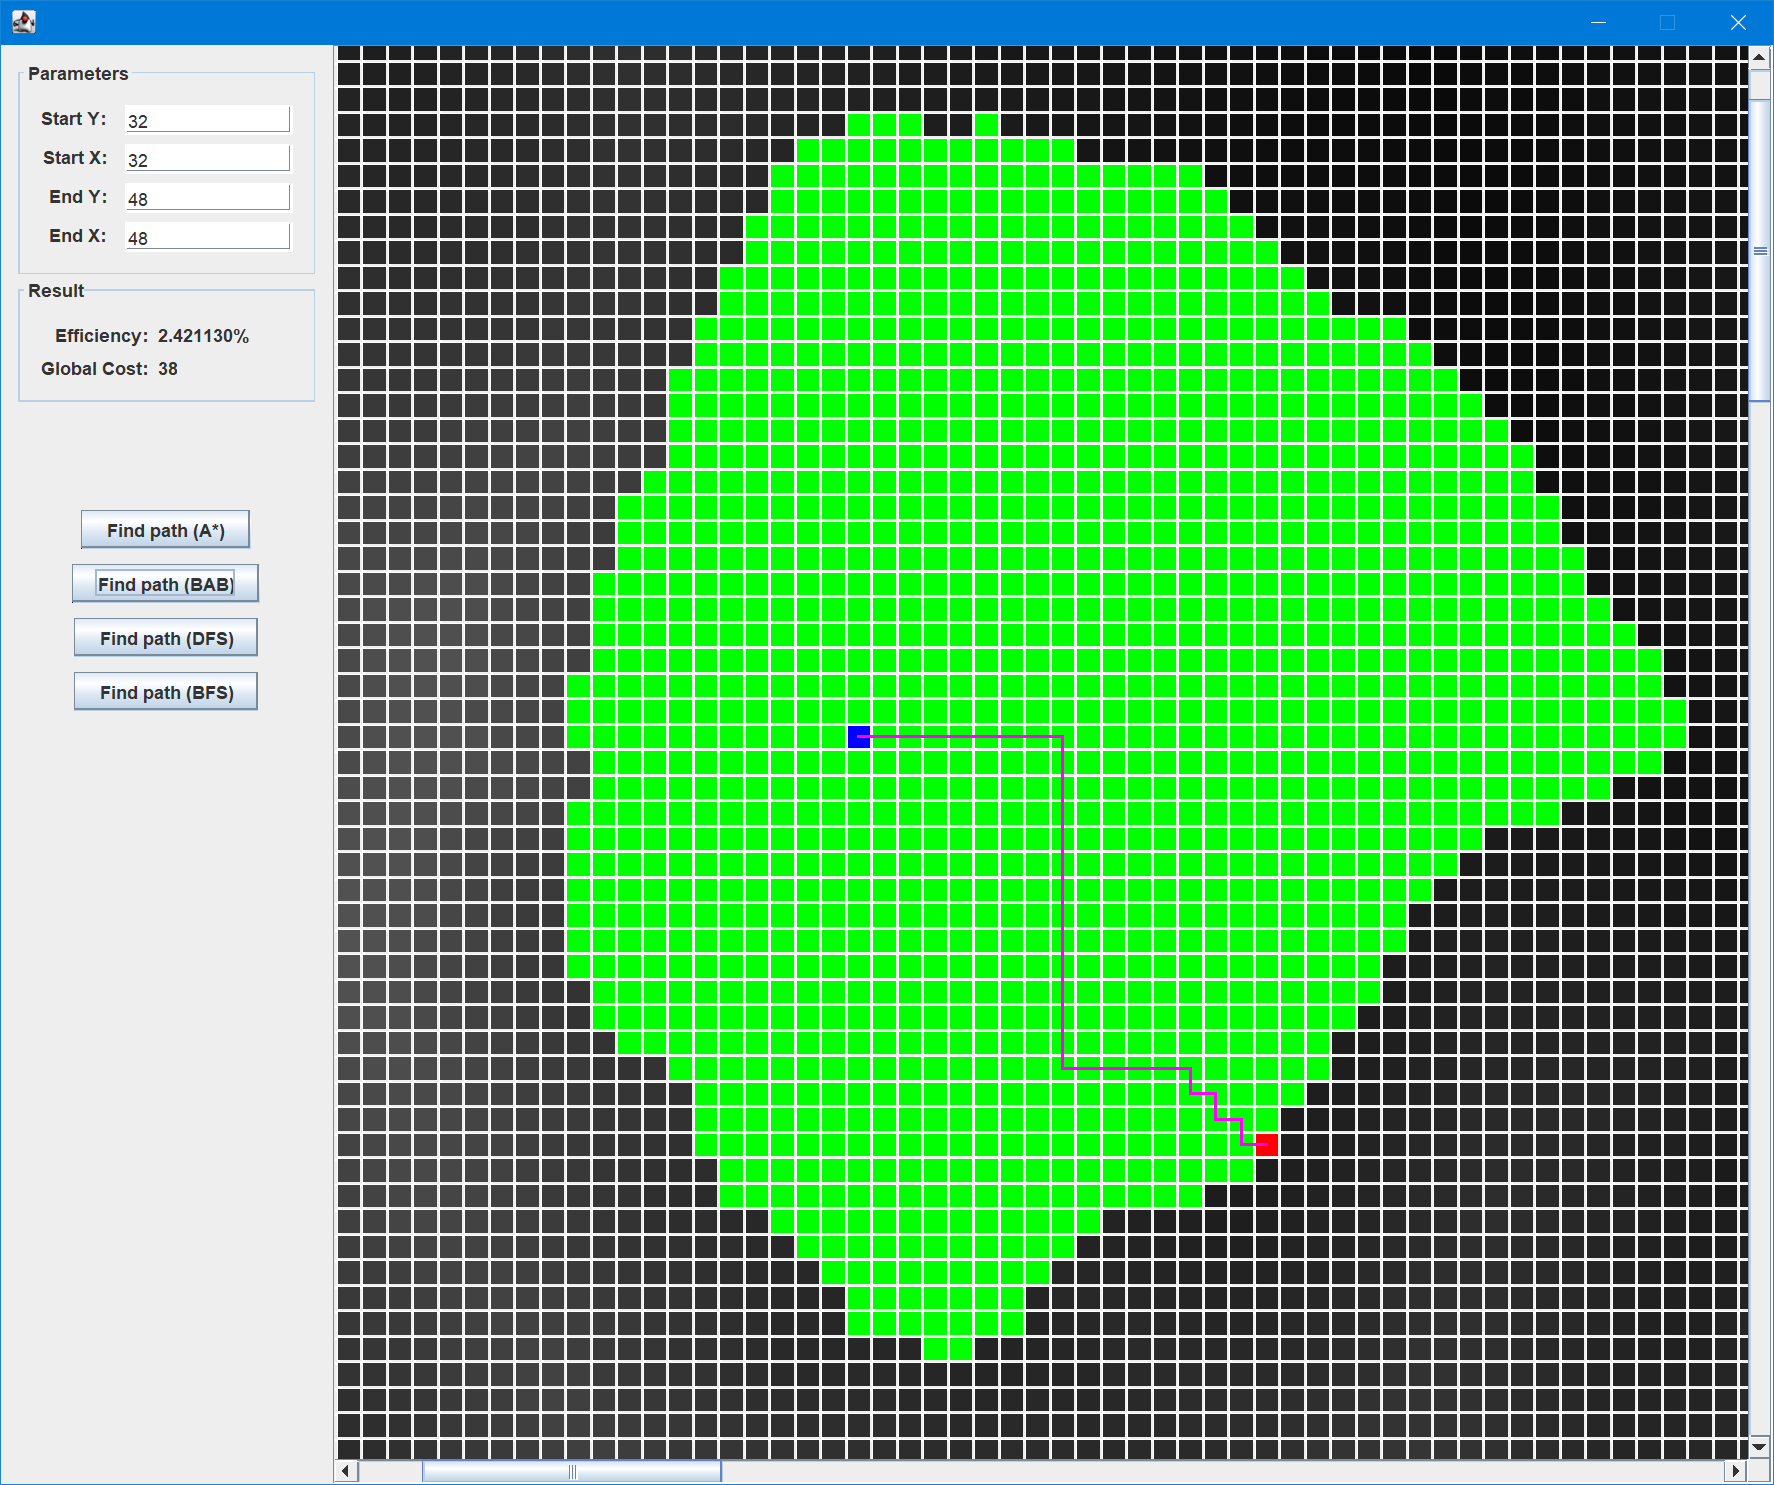
\includegraphics{./images/image-20210523072848208.png}
    \caption{}
    \end{figure}

    \begin{figure}
    \centering
    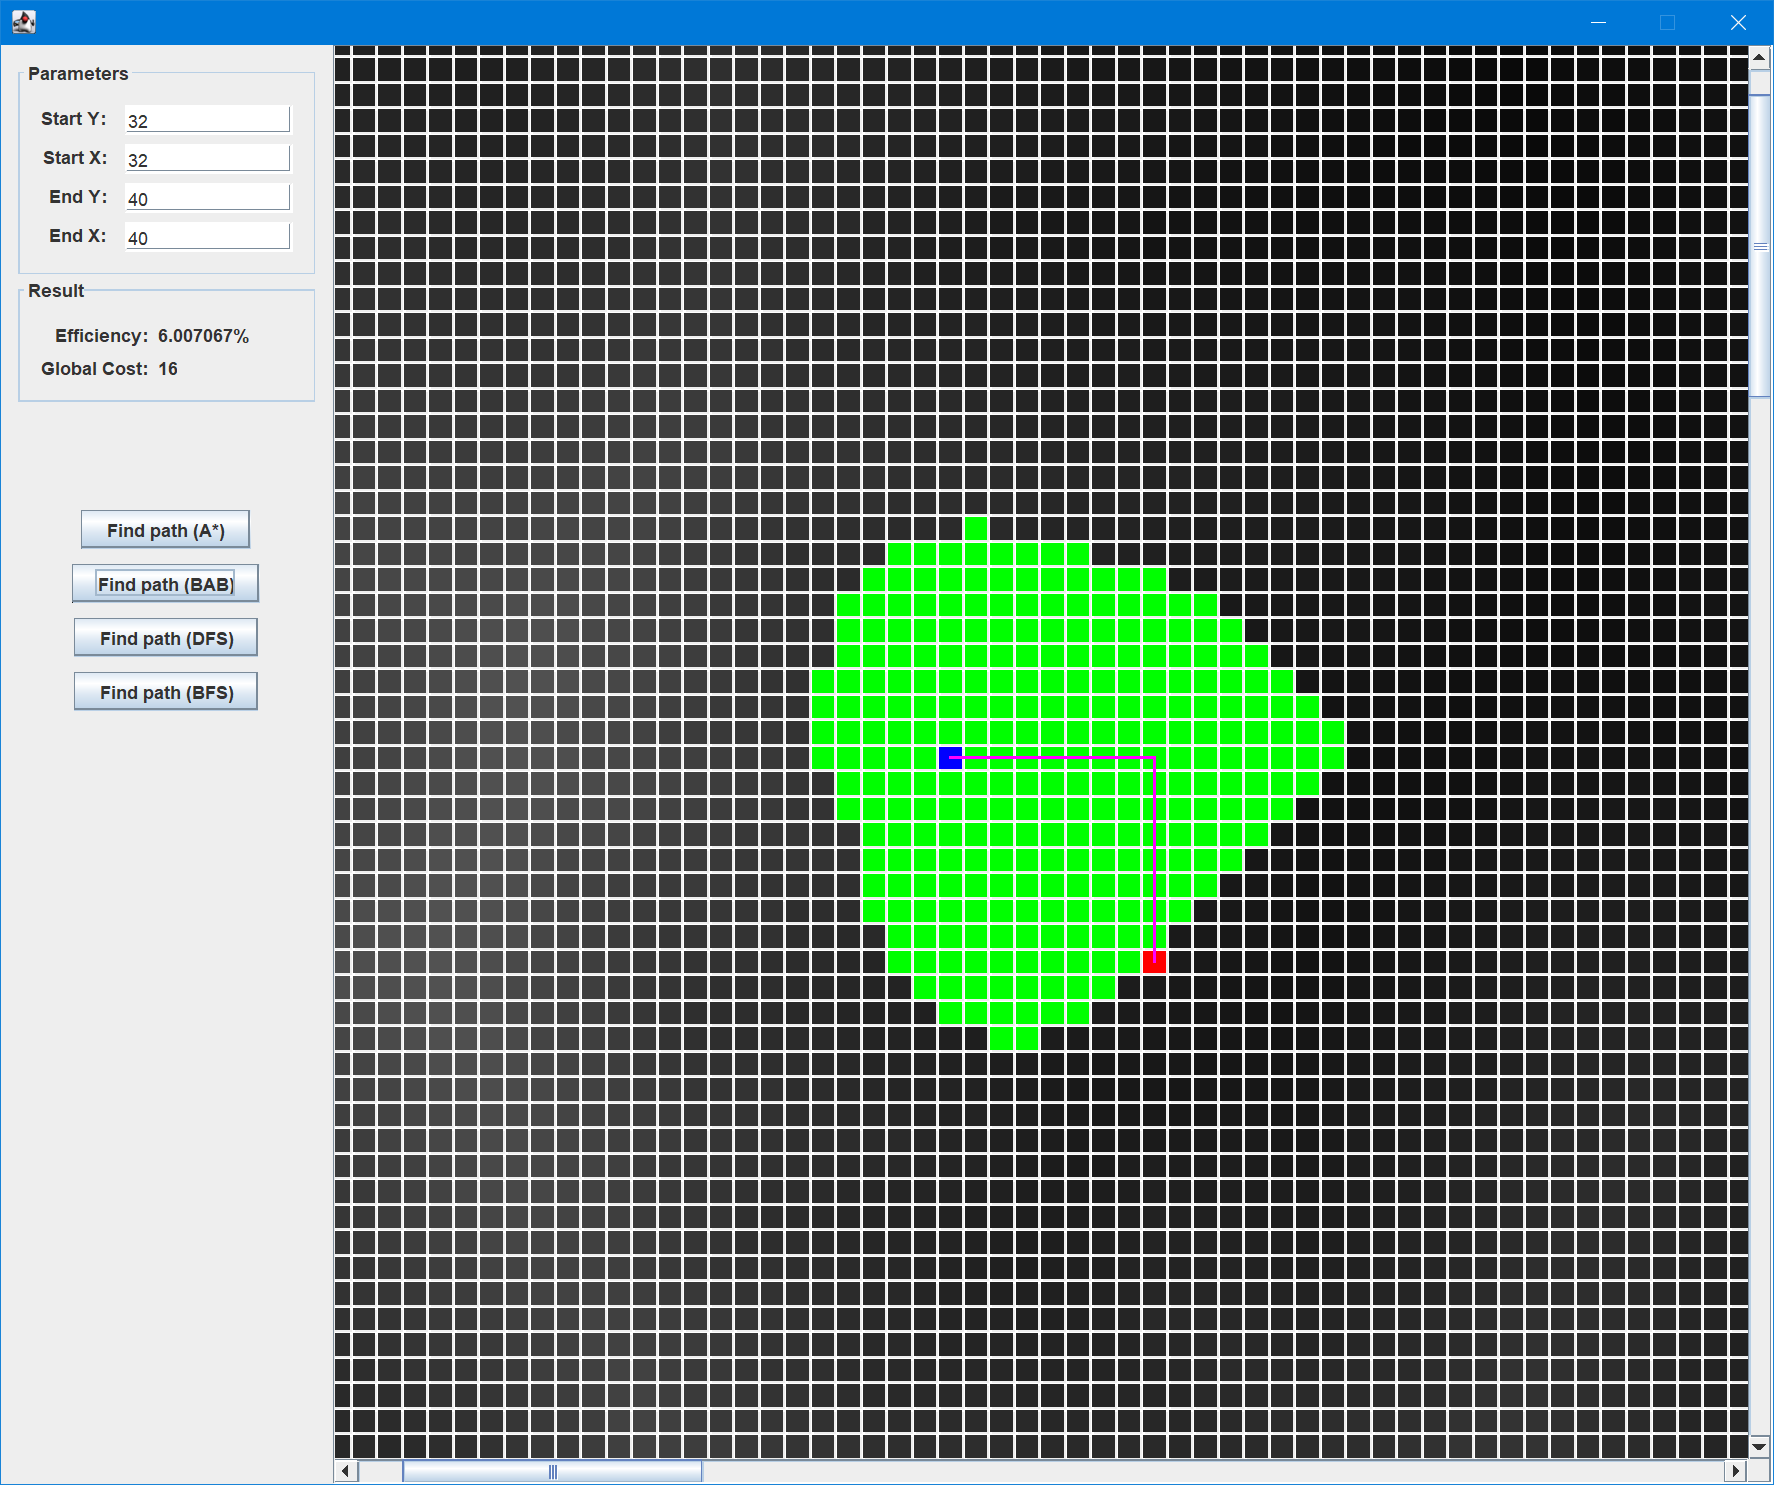
\includegraphics{./images/image-20210523072945713.png}
    \caption{}
    \end{figure}
  \end{itemize}
\end{itemize}

It can be seen from the above groups of experiments that the final
\emph{efficiency} of the \emph{branch-and-bound} algorithm has little to
do with the length of the path. Combining this \emph{branch-and-bound}
realization idea, the more complex the local shape, the lower the
\emph{efficiency}, which has a lot to do with the greedy idea used in
this algorithm. The greedy algorithm is to obtain the global optimal
solution by finding the local optimal solution. In our algorithm
implementation, we give priority to the node with the smallest
\emph{local cost} in the \emph{open list}. Under this condition, when
there are multiple local areas near the path, and each area has a small
or the same cost difference with other areas, the greedy algorithm will
be guided by this local optimal solution, thus performing a large number
of additional calculations. , Although these local optimal solutions may
be far from the global optimal solution.

\hypertarget{header-n406}{%
\subsection{Assessing the efficiency of my A* search
algorithm}\label{header-n406}}

Use the same experiment as the previous topic, but use the A* version of
the algorithm

\begin{itemize}
\item
  Experiment 1

  \begin{itemize}
  \item
    Experimental results:

    \begin{itemize}
    \item
      Heuristic algorithm based on Manhattan distance

      \begin{figure}
      \centering
      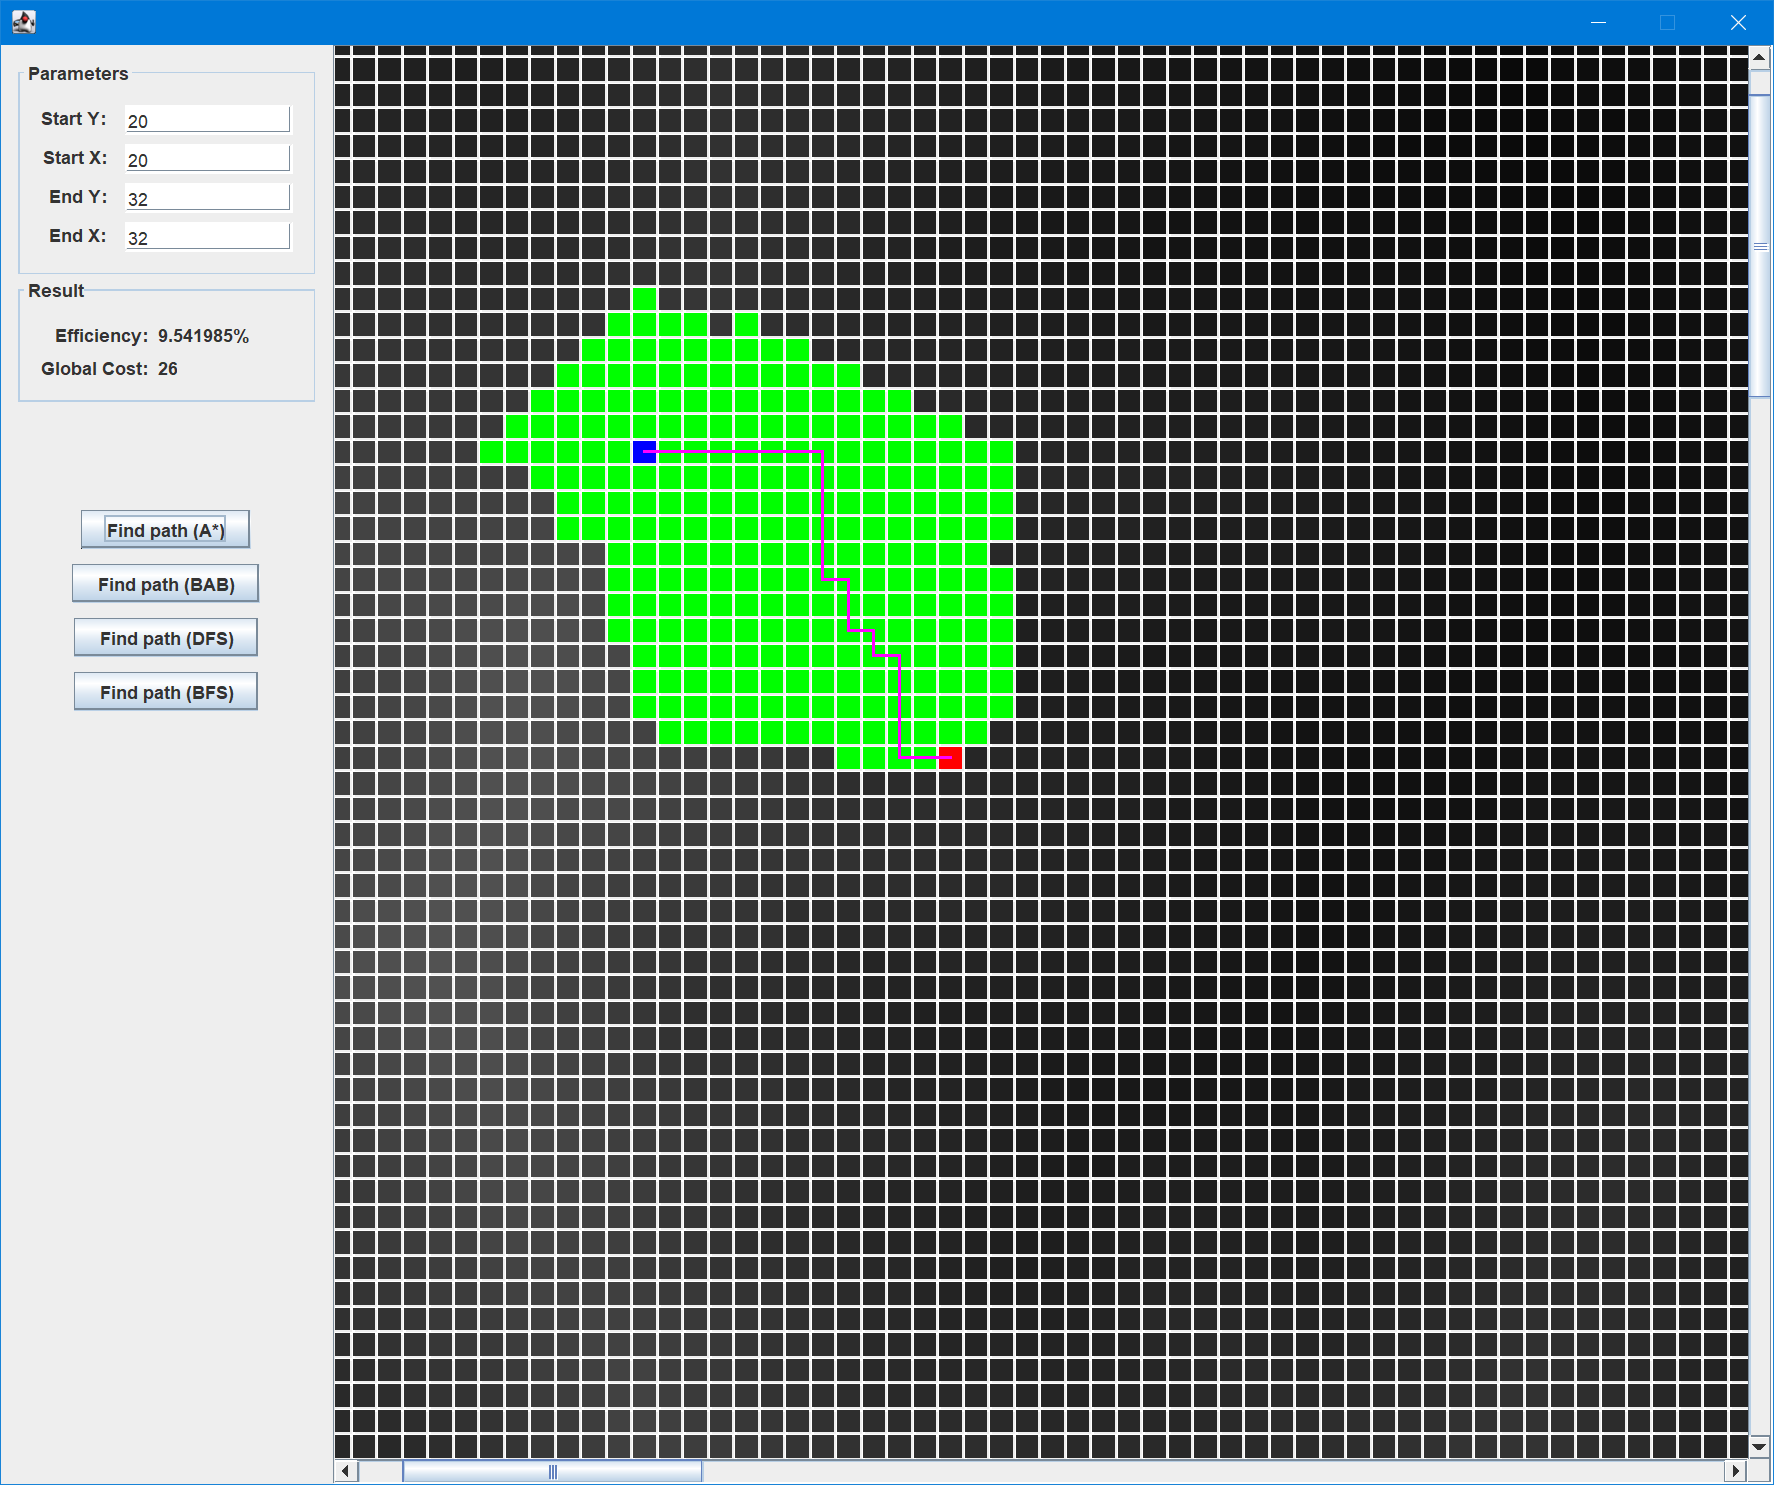
\includegraphics{./images/image-20210523082215544.png}
      \caption{}
      \end{figure}
    \item
      Heuristic algorithm based on Euclidean distance

      \begin{figure}
      \centering
      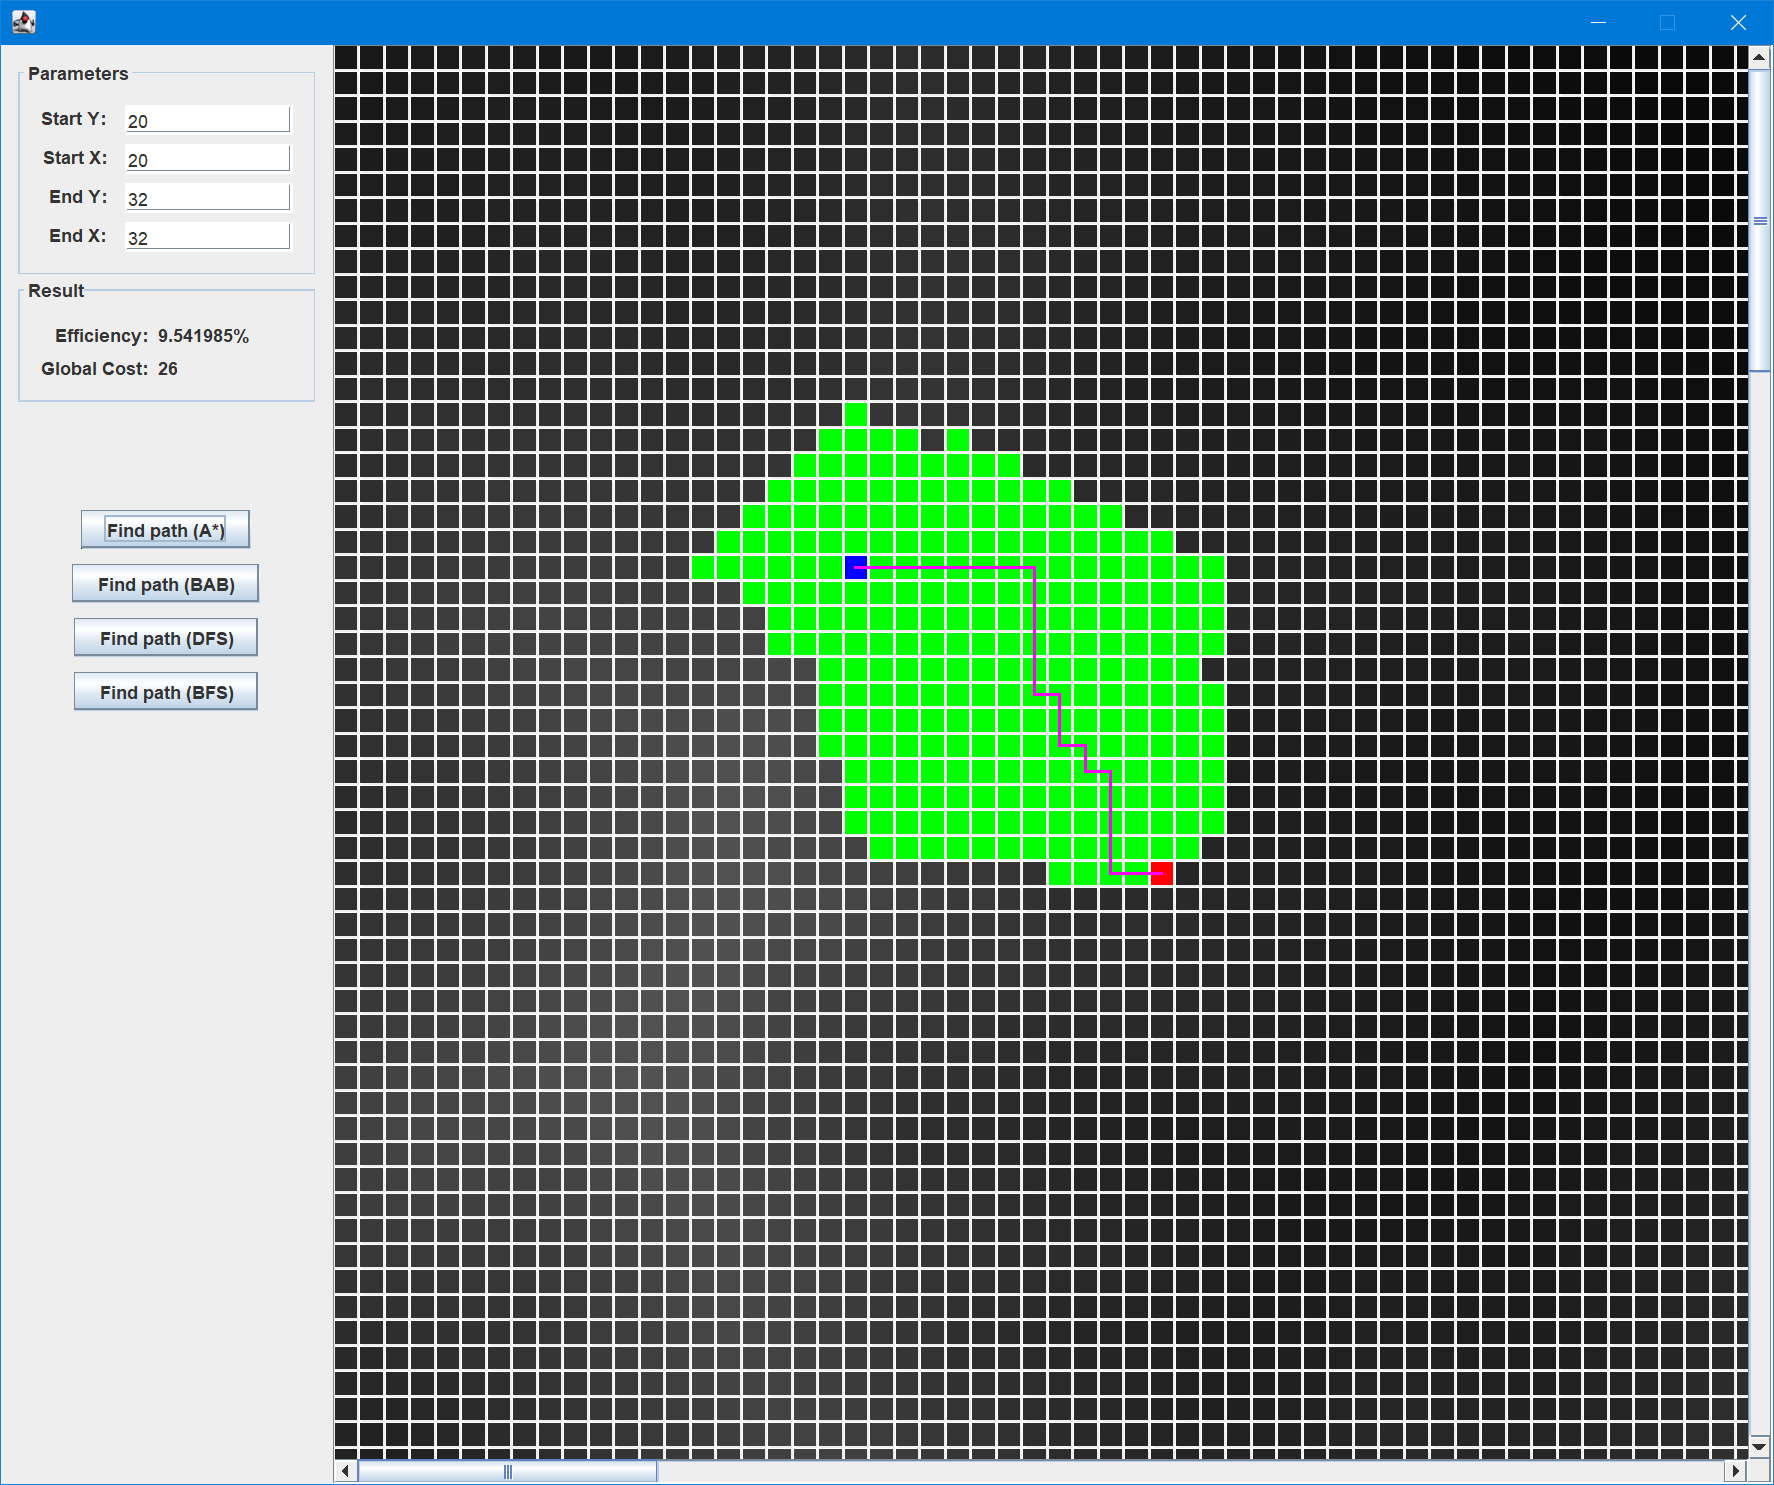
\includegraphics{./images/image-20210523082848030.png}
      \caption{}
      \end{figure}
    \end{itemize}
  \end{itemize}
\item
  Experiment 2

  \begin{itemize}
  \item
    Experimental results:

    \begin{itemize}
    \item
      Heuristic algorithm based on Manhattan distance

      \begin{figure}
      \centering
      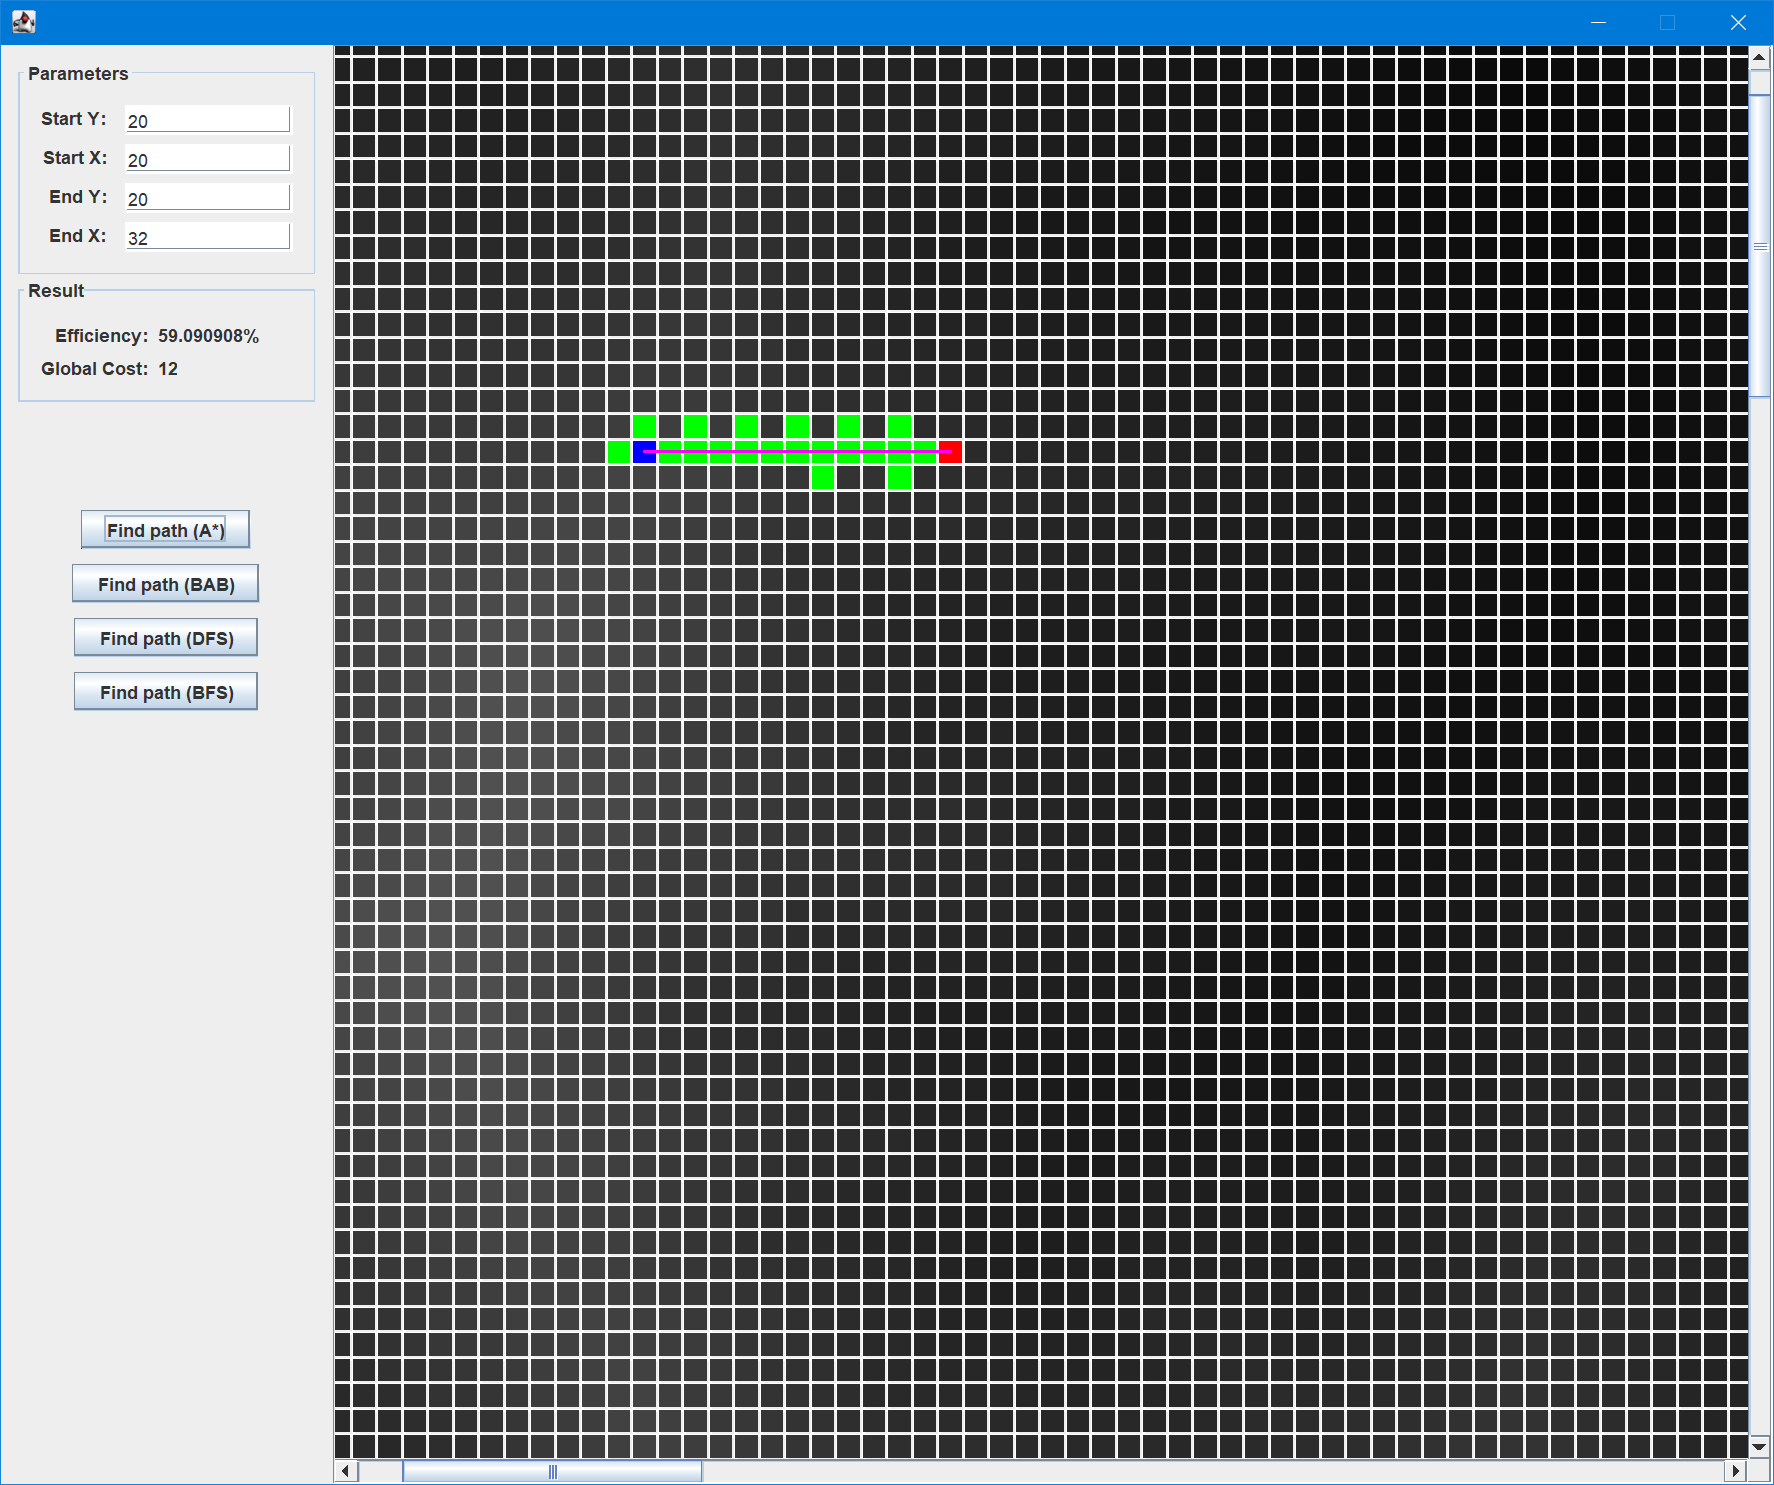
\includegraphics{./images/image-20210523082247436.png}
      \caption{}
      \end{figure}

      \begin{figure}
      \centering
      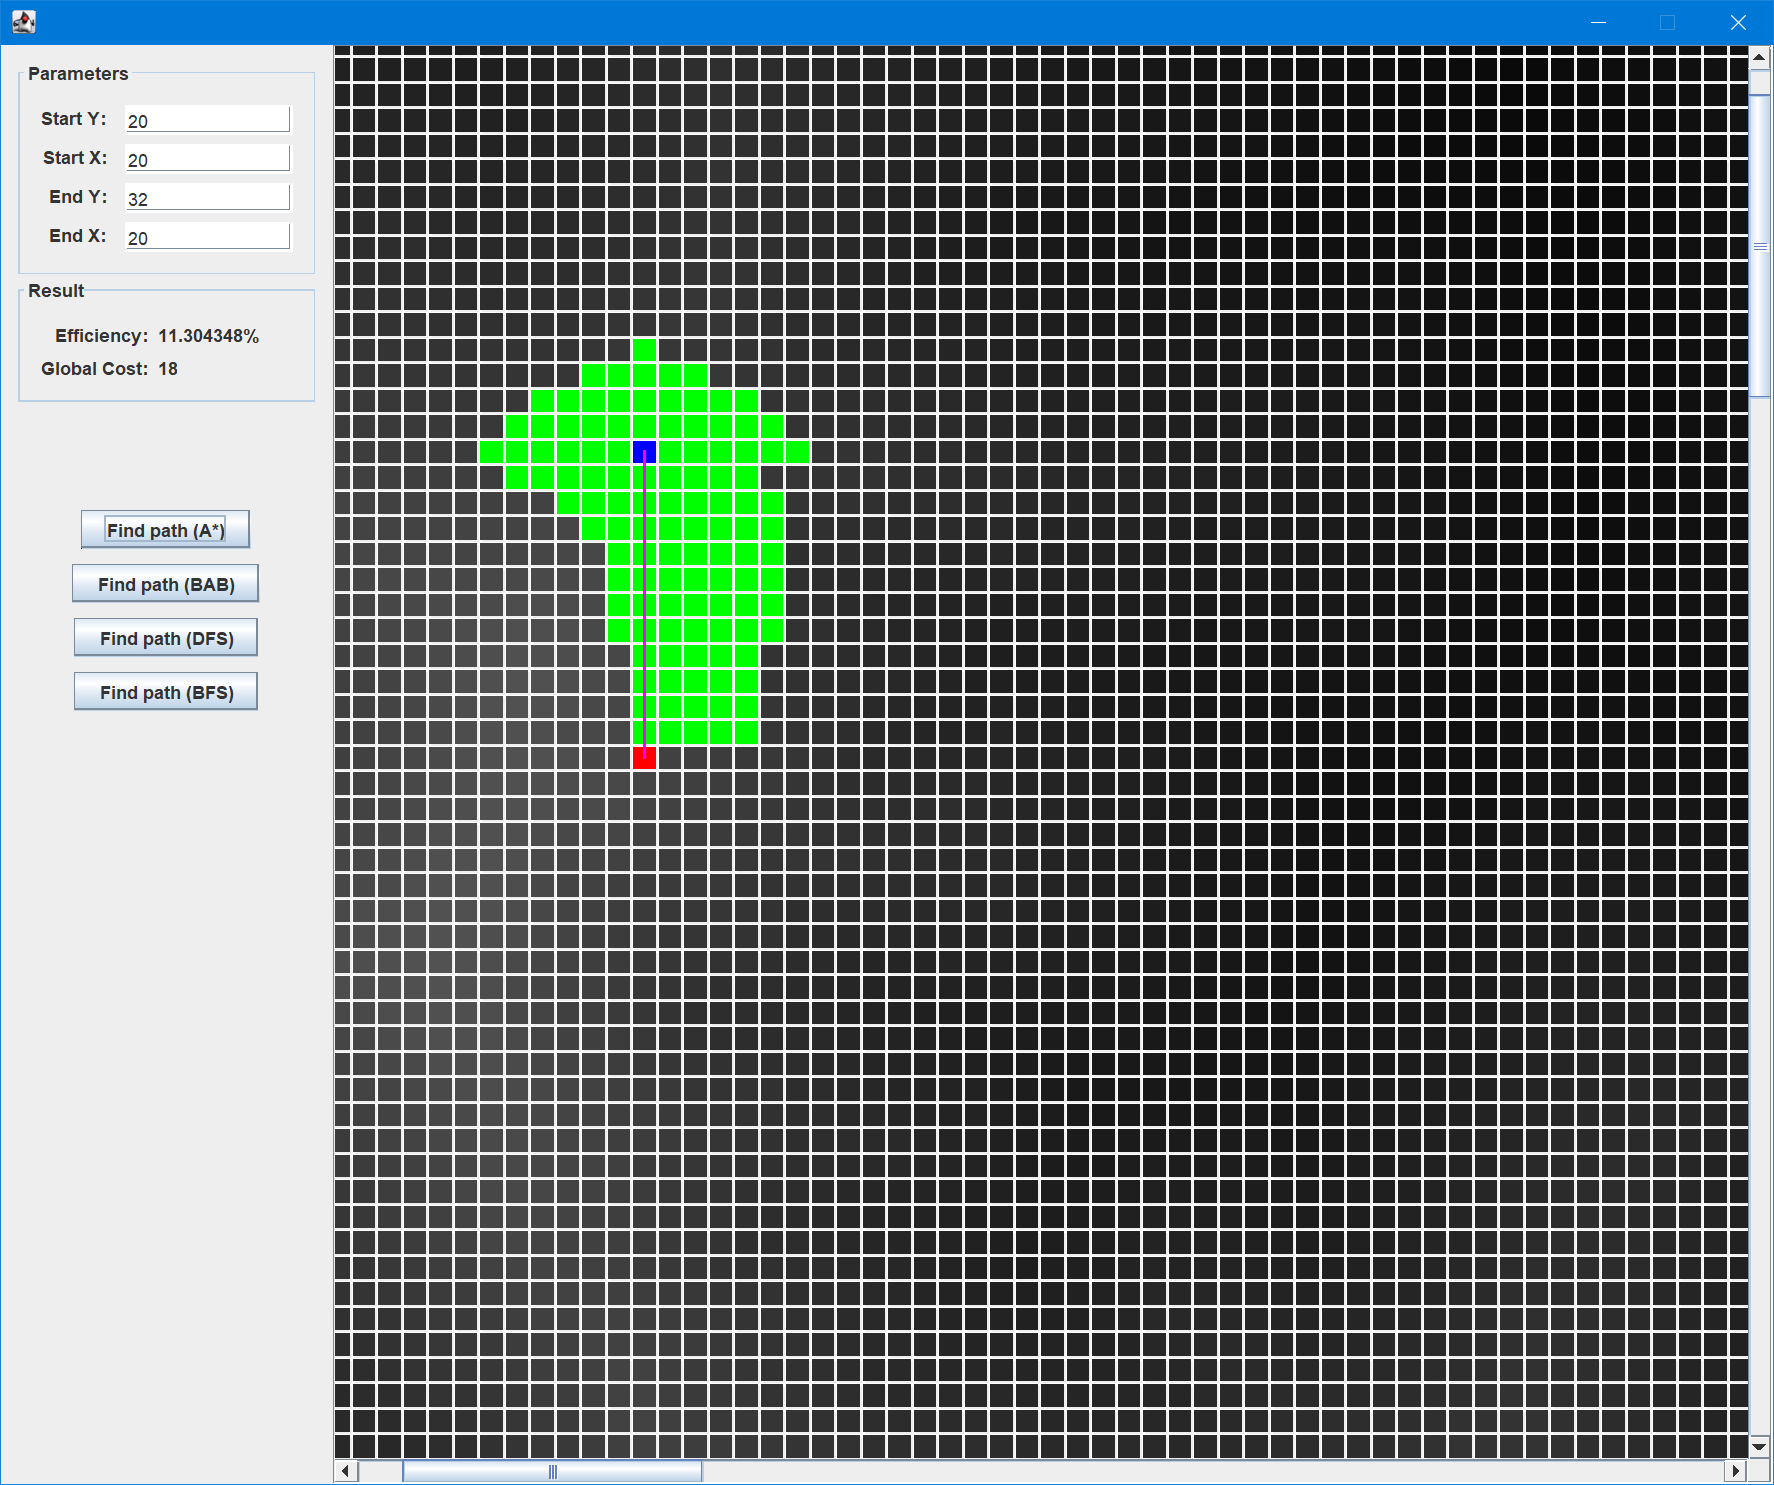
\includegraphics{./images/image-20210523082304339.png}
      \caption{}
      \end{figure}
    \item
      Heuristic algorithm based on Euclidean distance

      \begin{figure}
      \centering
      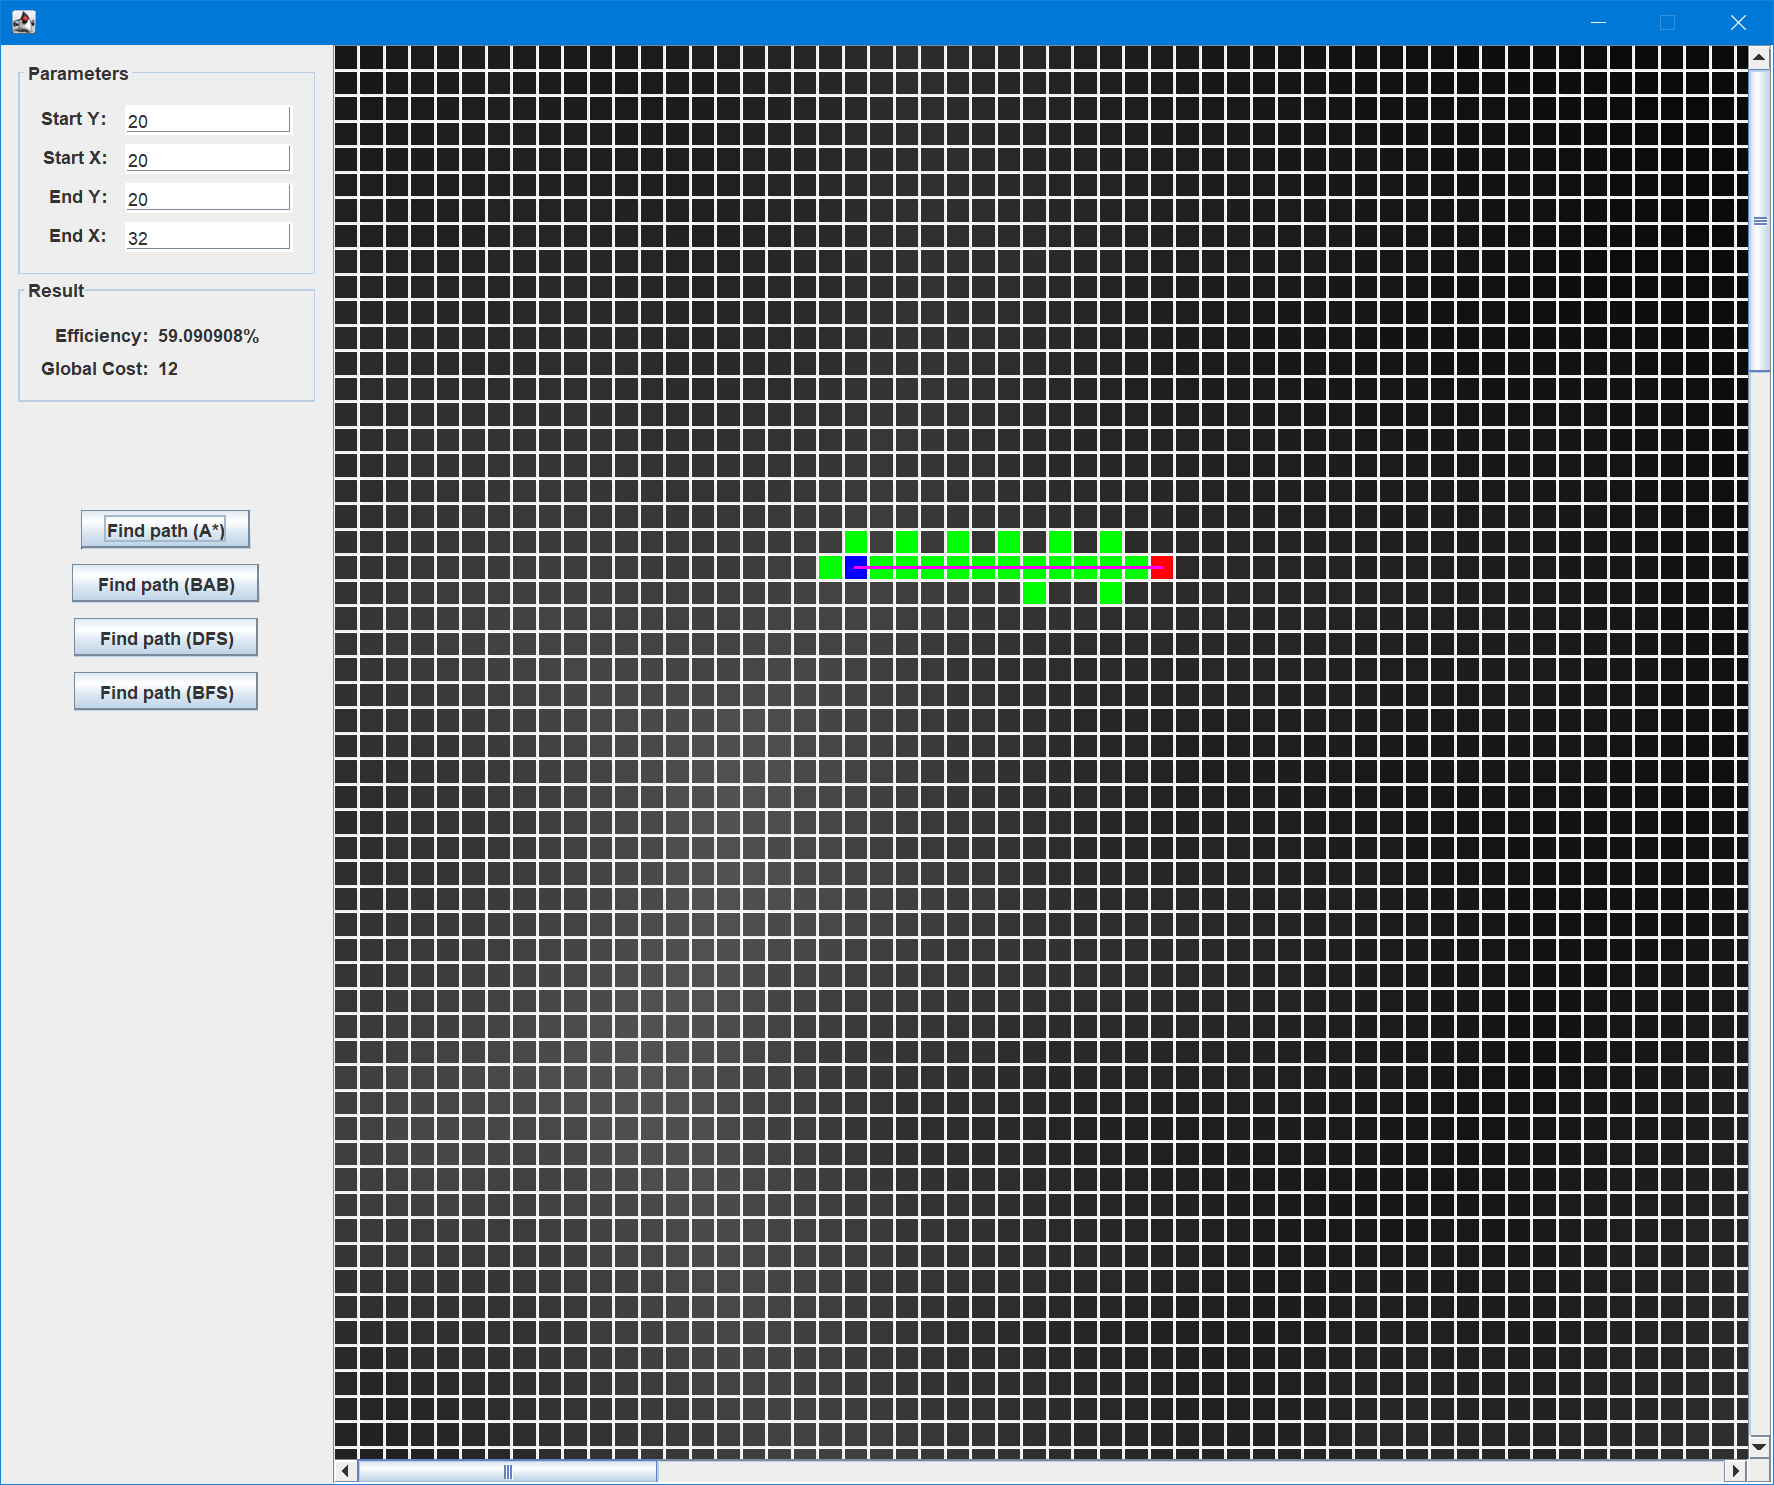
\includegraphics{./images/image-20210523083212866.png}
      \caption{}
      \end{figure}

      \begin{figure}
      \centering
      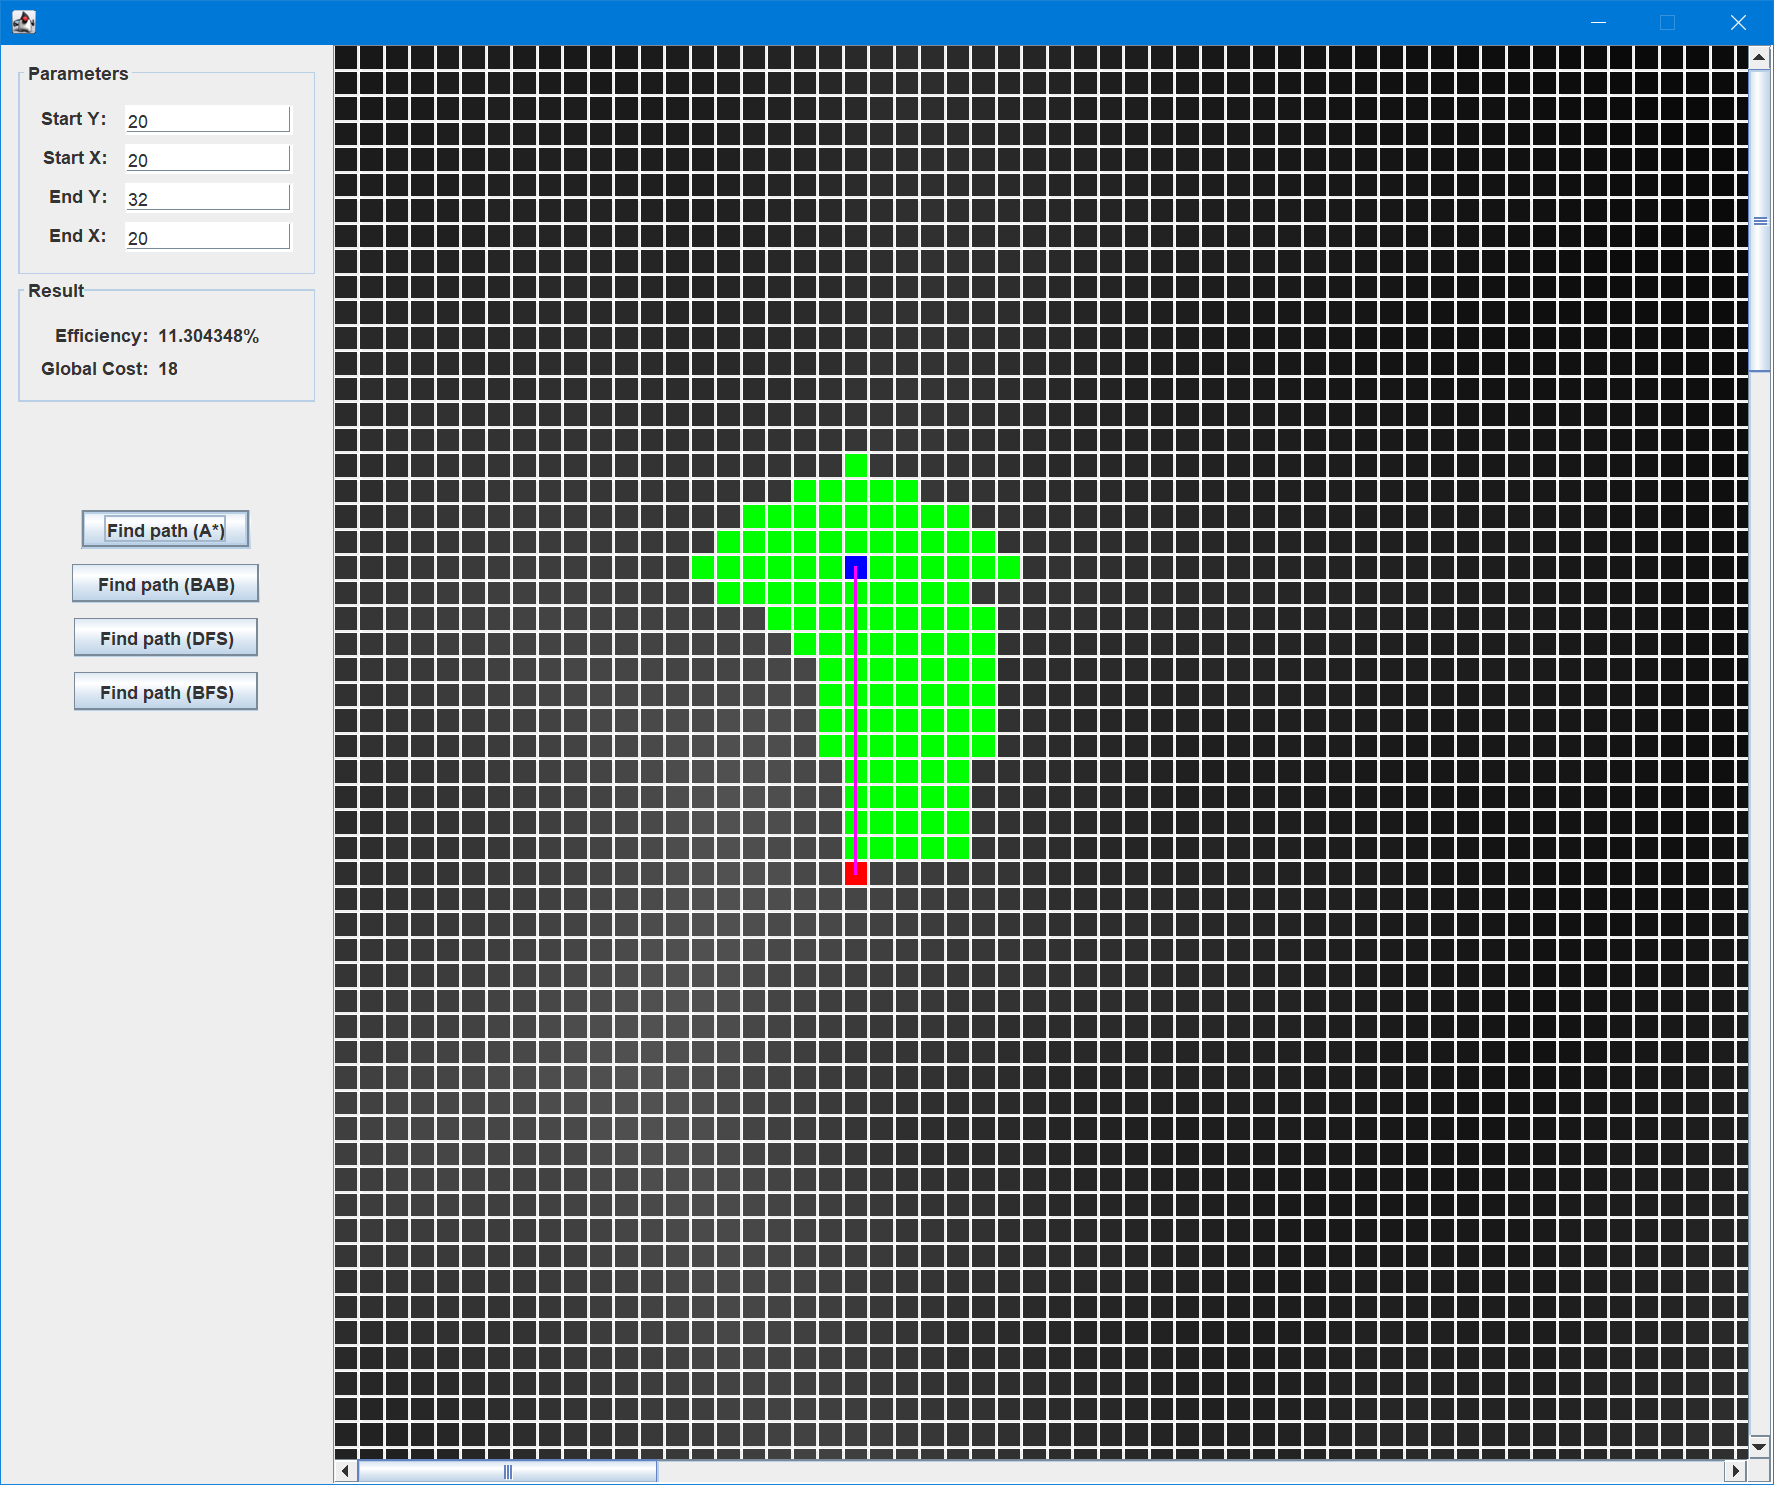
\includegraphics{./images/image-20210523083225750.png}
      \caption{}
      \end{figure}
    \end{itemize}
  \end{itemize}
\item
  Experiment 3

  \begin{itemize}
  \item
    Experimental results:

    \begin{itemize}
    \item
      Heuristic algorithm based on Manhattan distance

      \begin{figure}
      \centering
      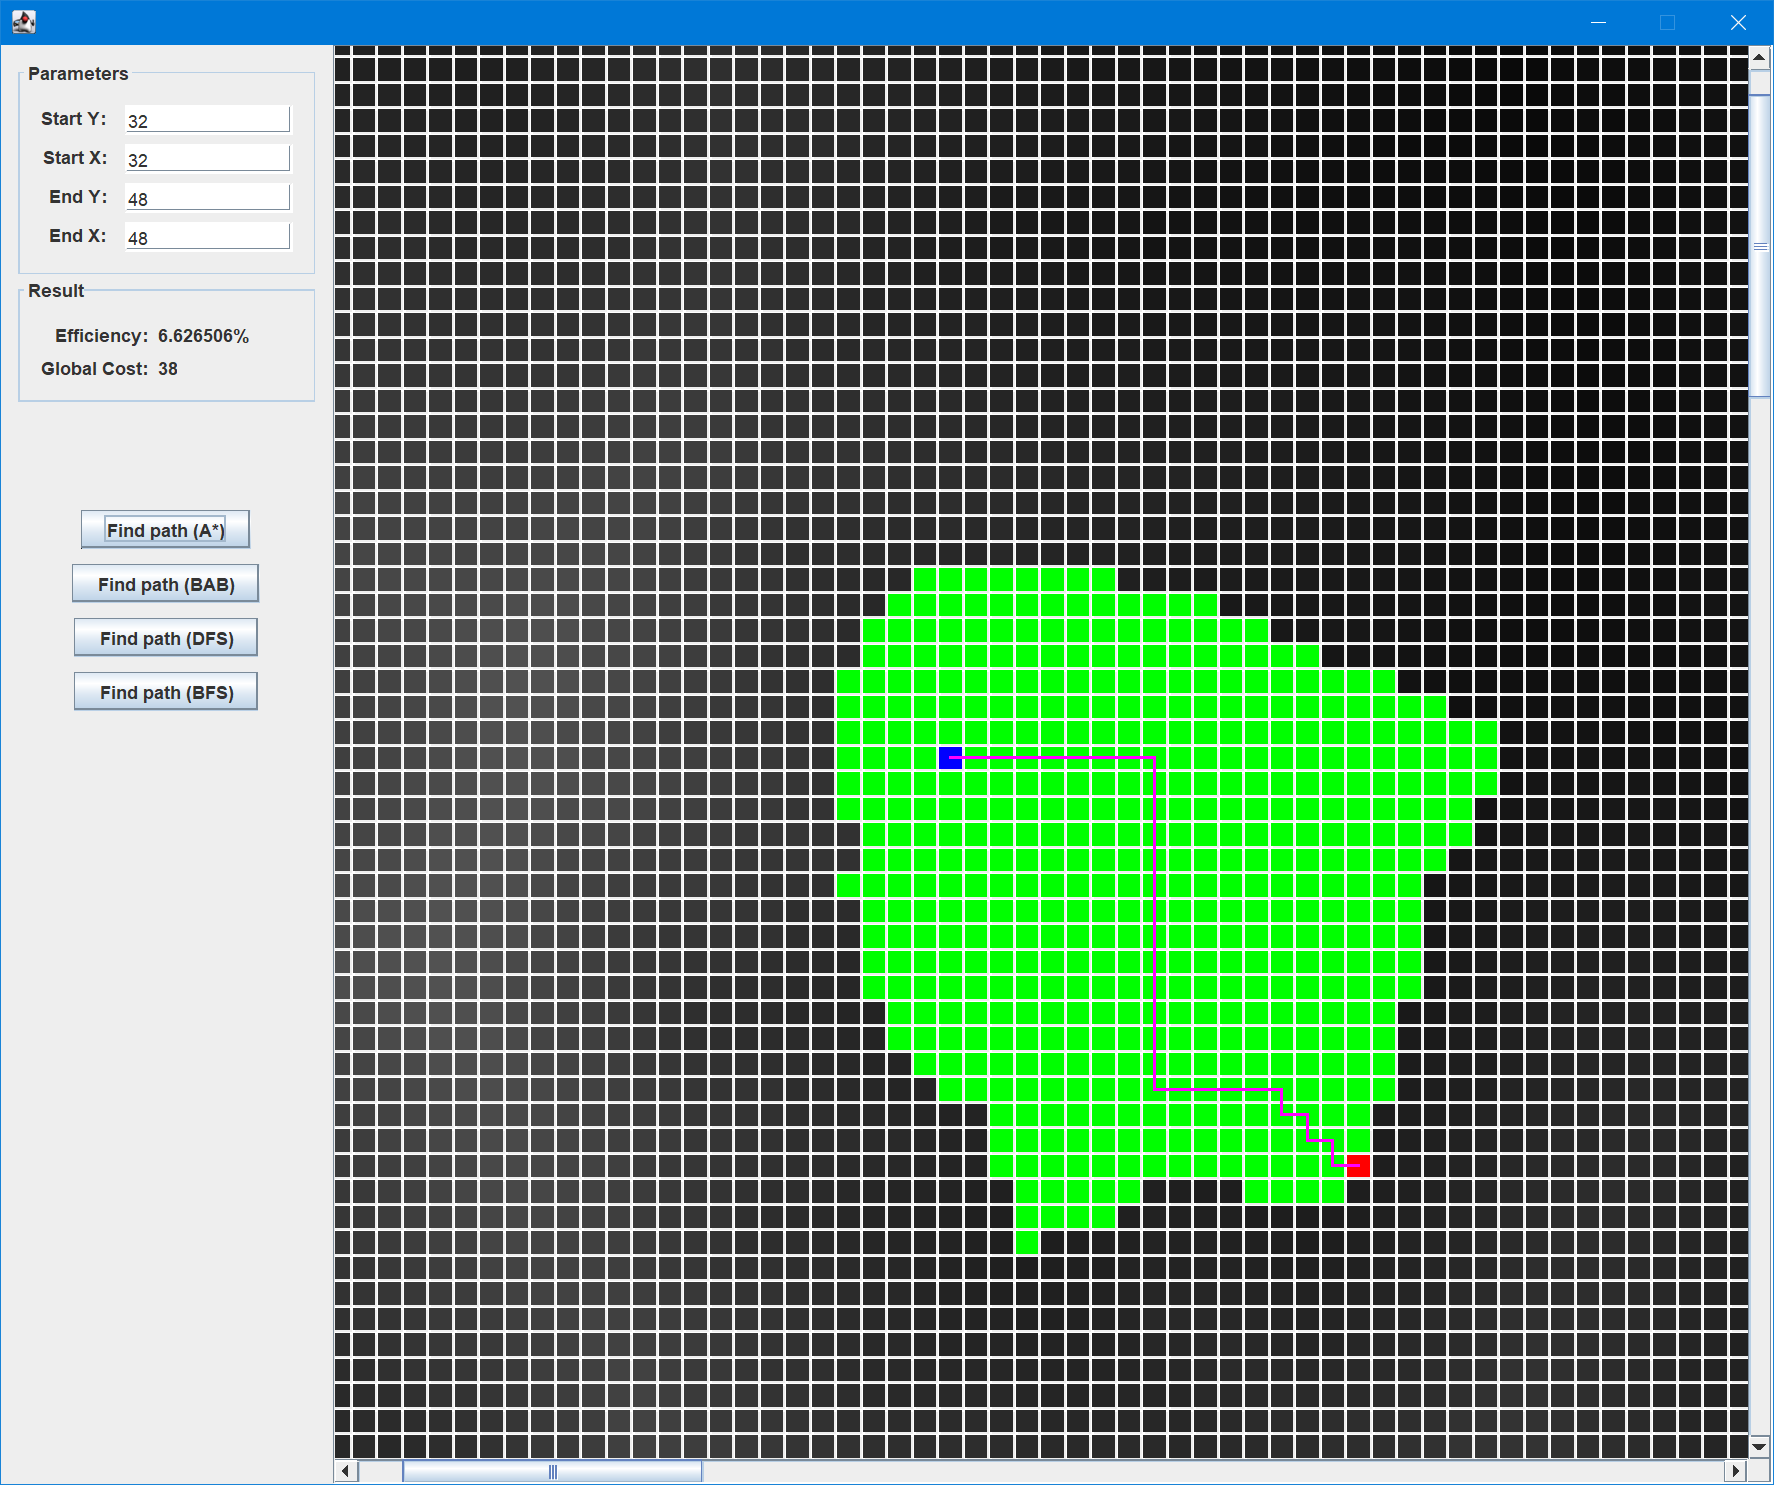
\includegraphics{./images/image-20210523082345704.png}
      \caption{}
      \end{figure}

      \begin{figure}
      \centering
      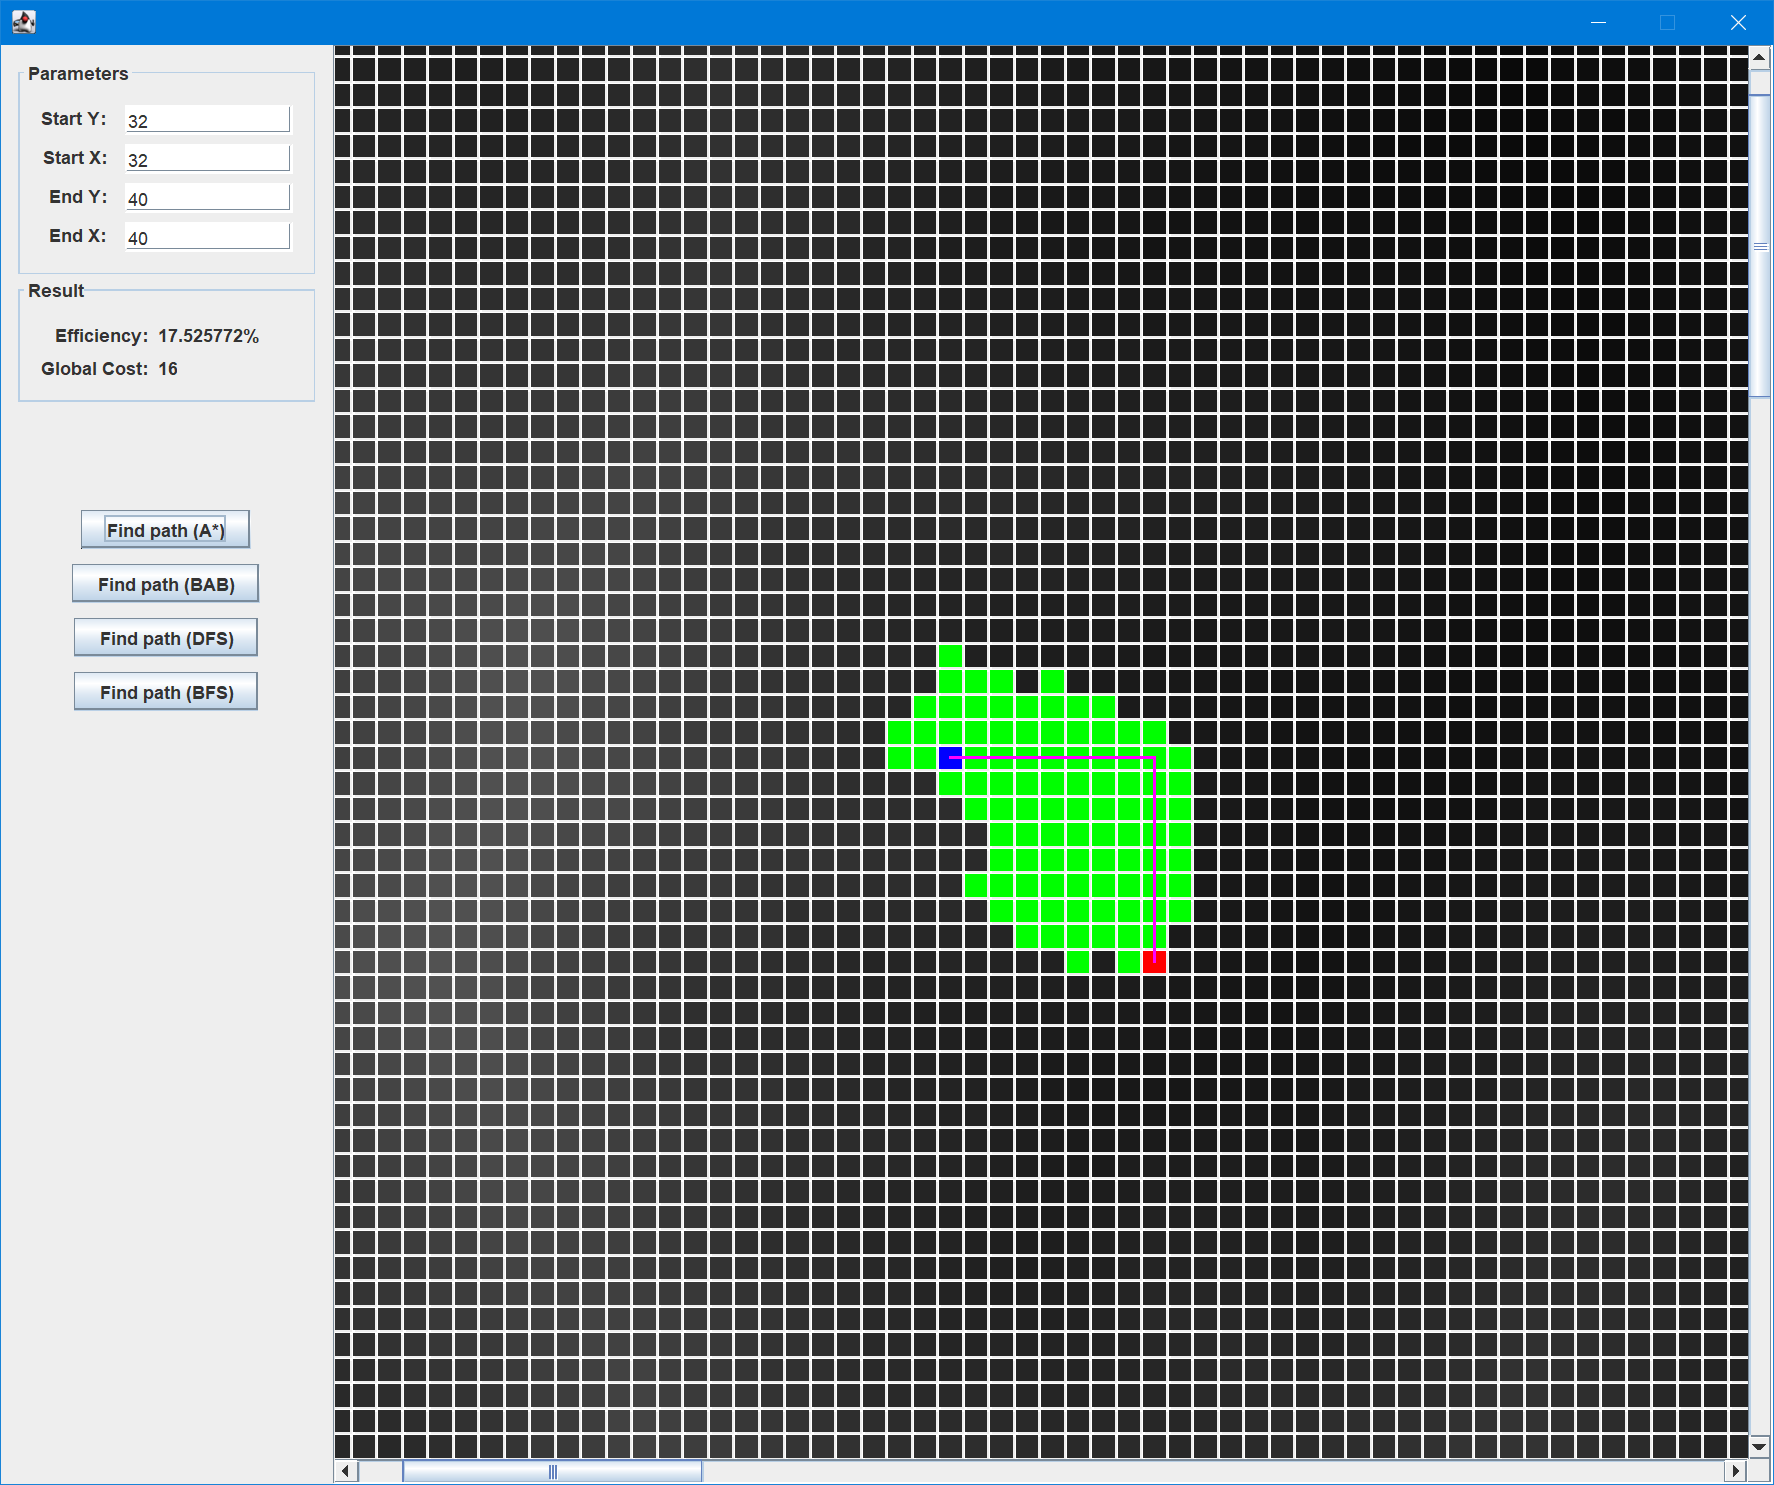
\includegraphics{./images/image-20210523082417053.png}
      \caption{}
      \end{figure}
    \item
      Heuristic algorithm based on Euclidean distance

      \begin{figure}
      \centering
      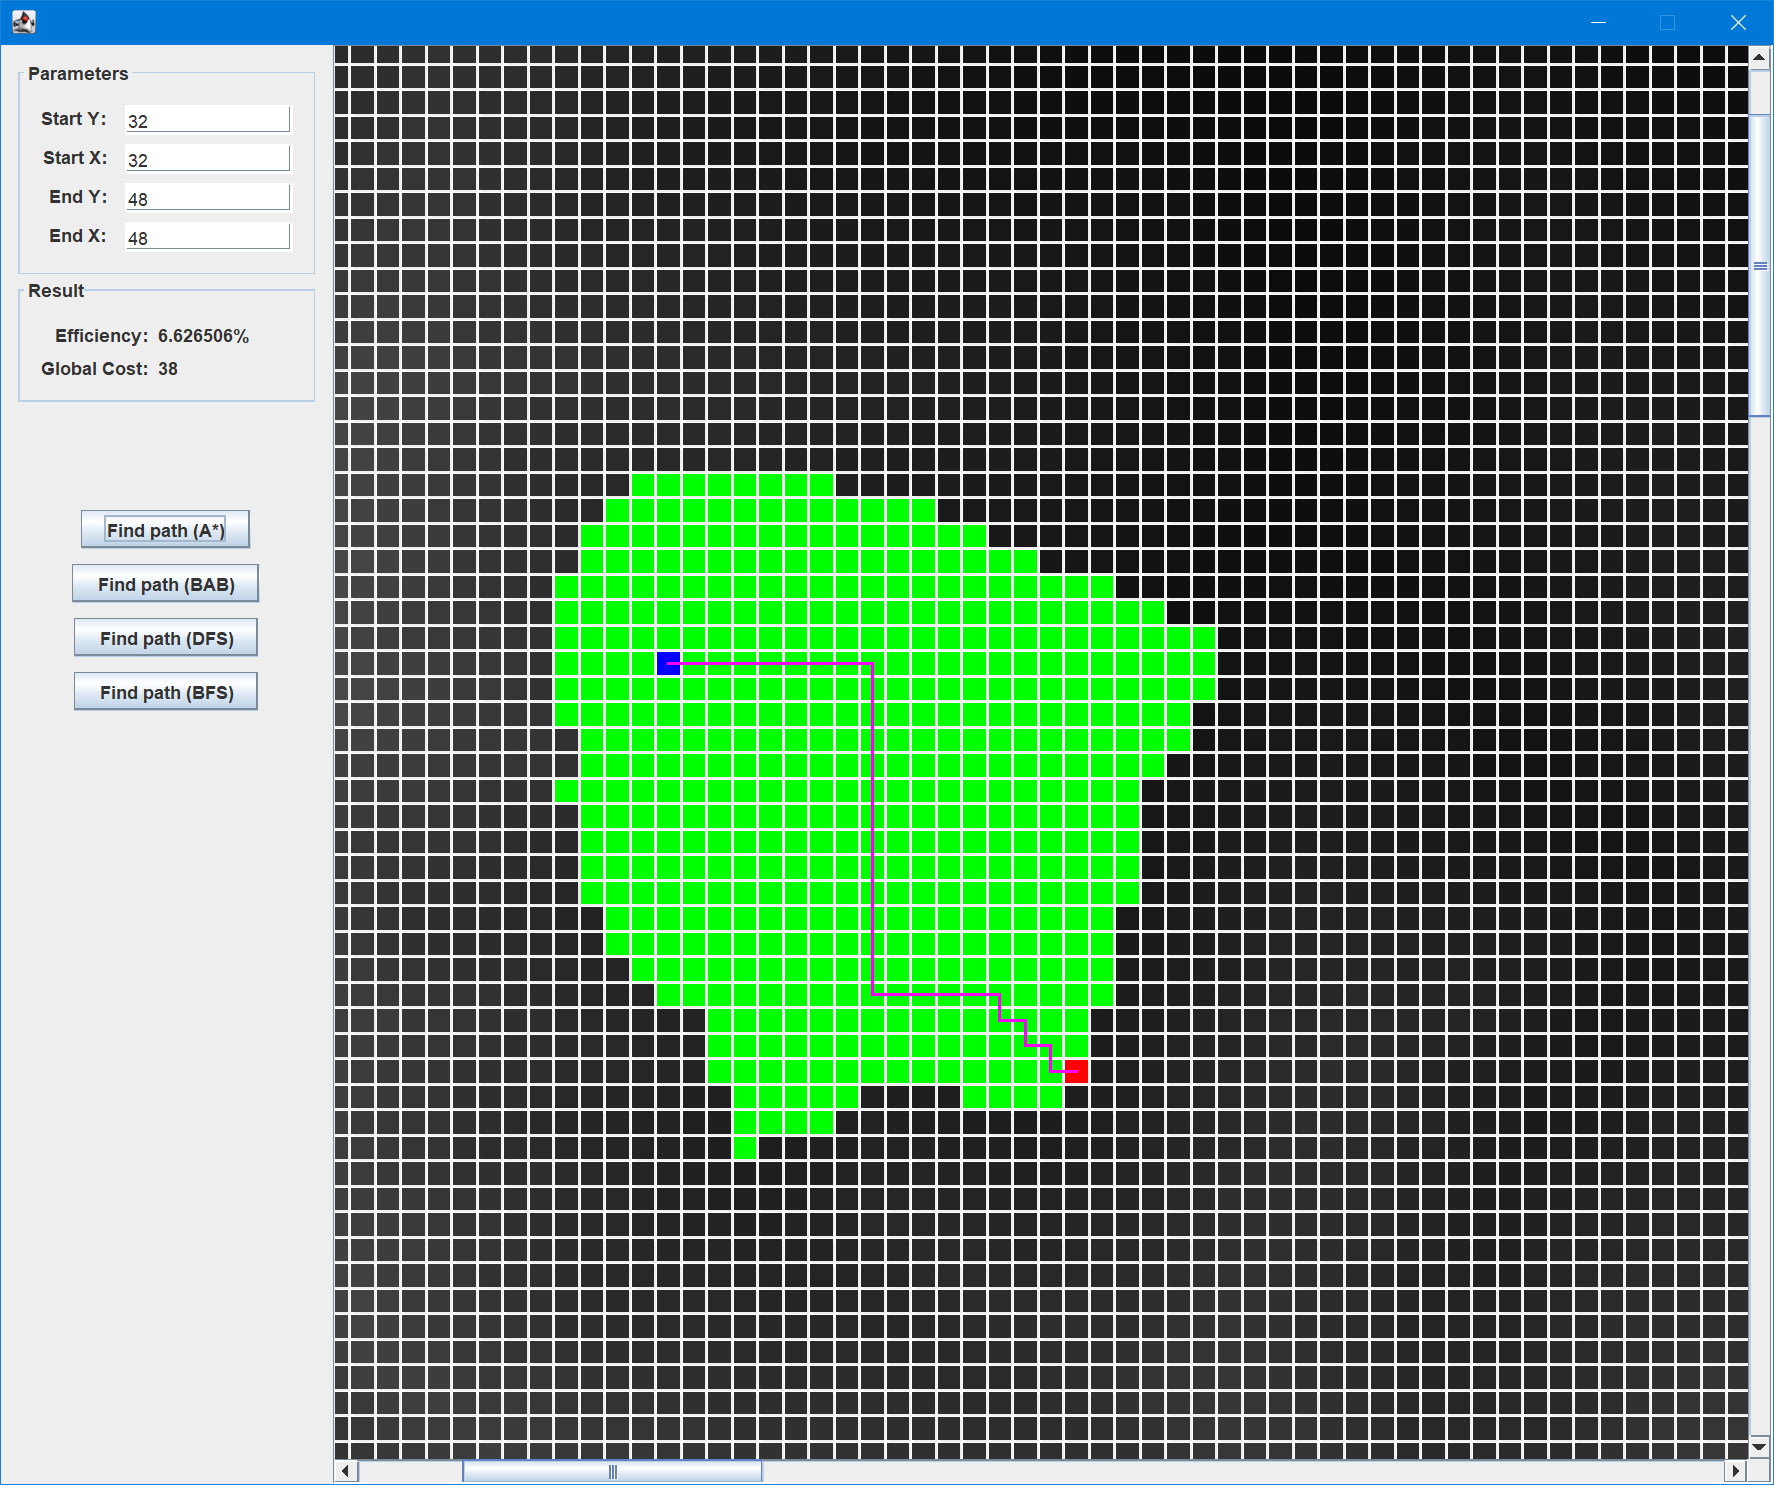
\includegraphics{./images/image-20210523083353747.png}
      \caption{}
      \end{figure}

      \begin{figure}
      \centering
      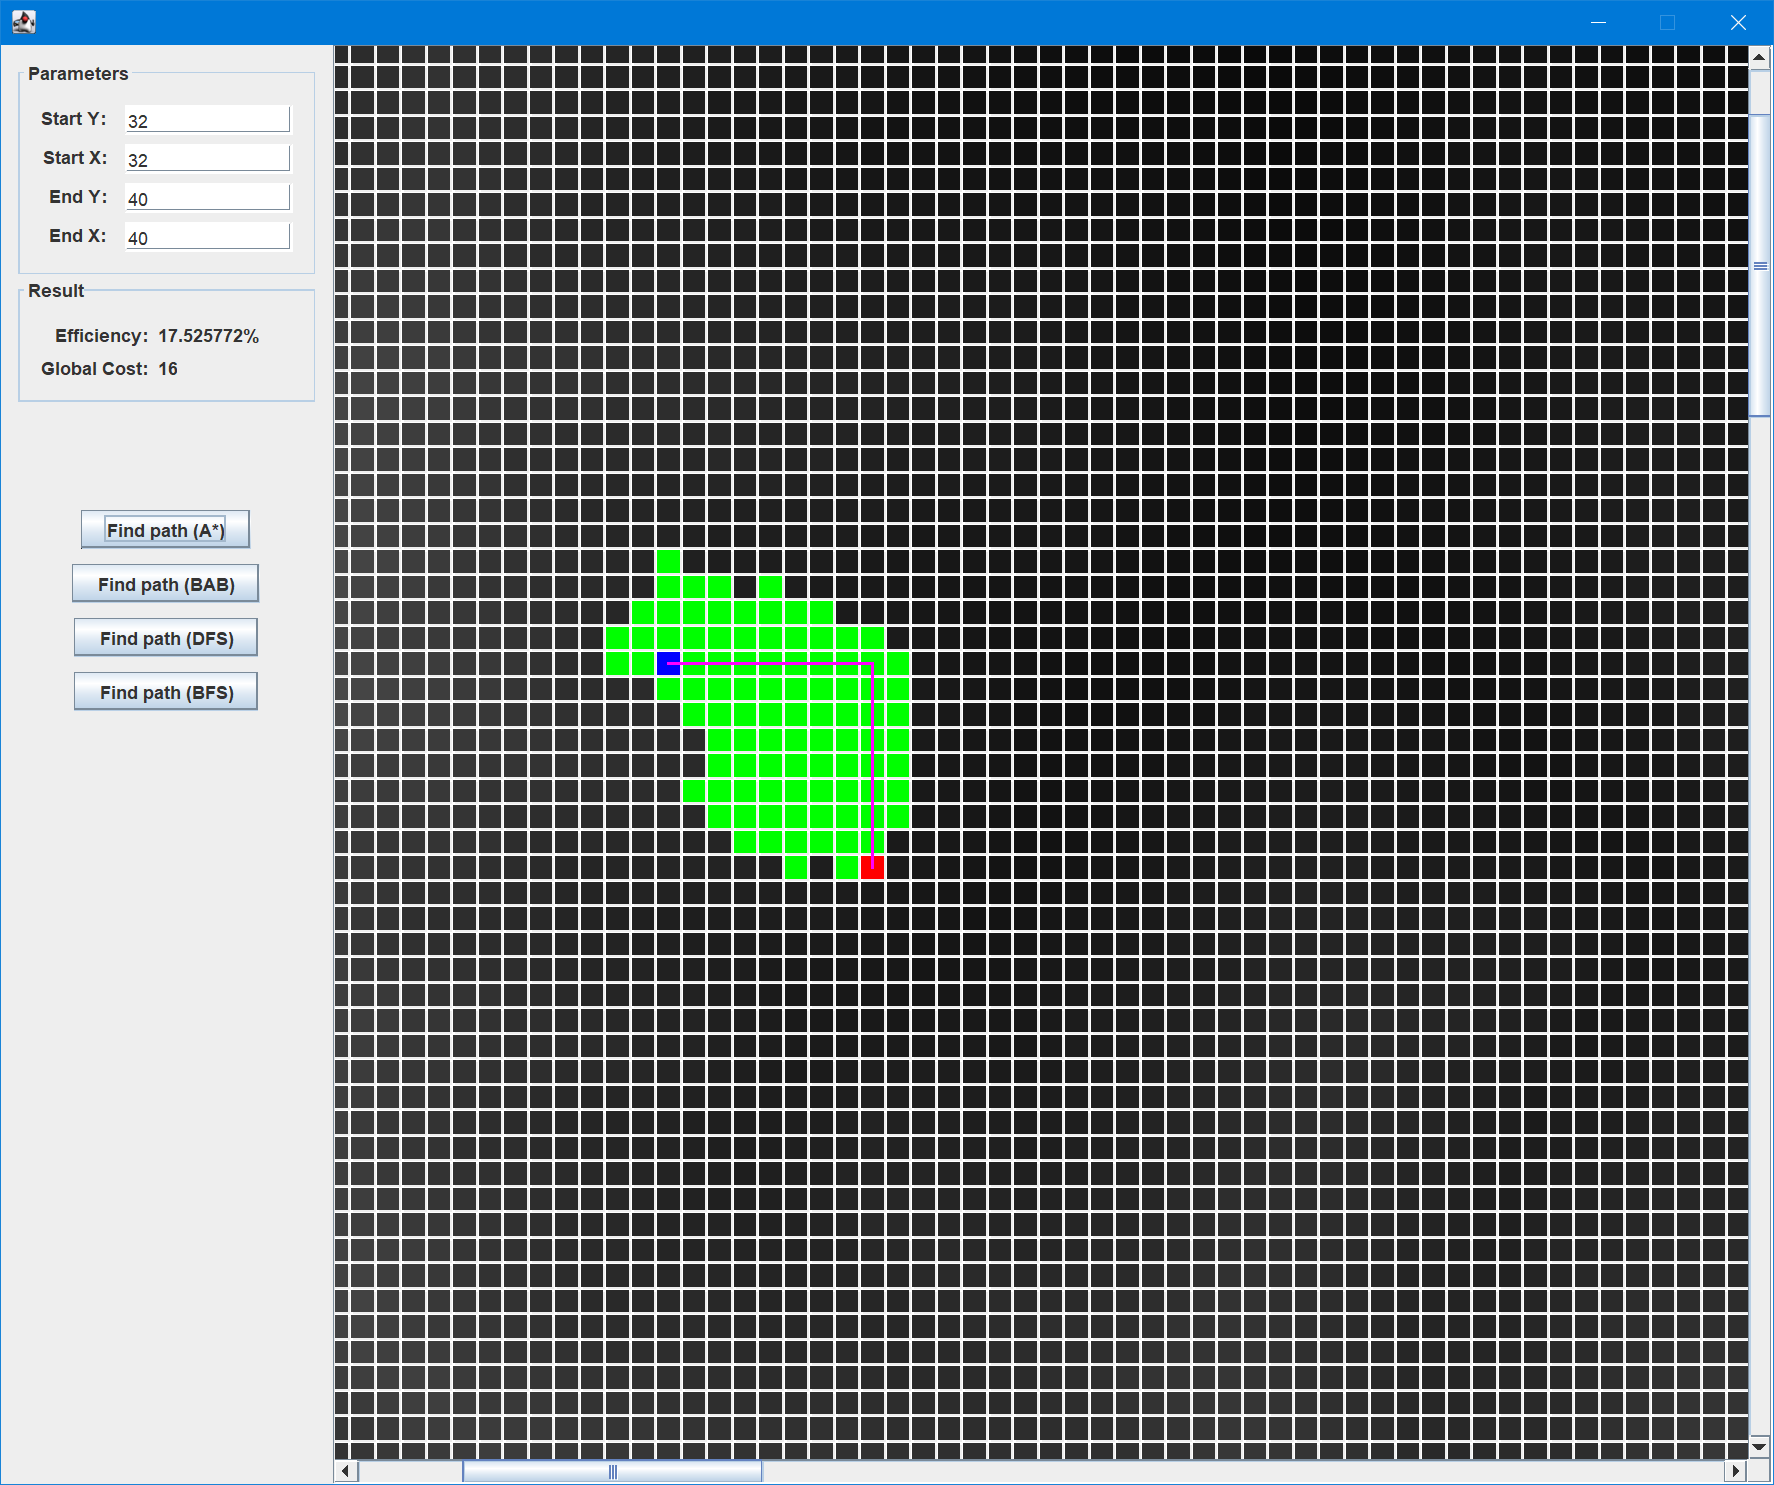
\includegraphics{./images/image-20210523083415438.png}
      \caption{}
      \end{figure}
    \end{itemize}
  \end{itemize}
\end{itemize}

Through the above groups of experiments, it can be seen that the
\emph{efficiency} of the *A\textbackslash** algorithm is better than the
\emph{branch-and-bound} algorithm in most cases, and the green square is
less than the \emph{branch-and-bound} algorithm in most cases It can
also be said that the *A\textbackslash** algorithm is closer to the
target more accurately than the \emph{branch-and-bound} algorithm. This
is due to its \emph{heuristic function}.

*A** When calculating the cost in the algorithm, the cost function can
be expressed as \(F = G + H \), where \(G\) represents the total cost
from the starting point to the current node, and \(H\) is called the
heuristic function, which means from the current node Estimate of the
remaining cost to the target node. *A** When the algorithm selects the
next node, the node with the smallest estimated value \(H\) will be
selected first. Therefore, the selection of the heuristic function \(H\)
has an absolute impact on the final efficiency of the *A** algorithm.
The \textbf{*A\textbackslash{}} algorithm will search along the gradient
direction of the heuristic function \(H\). A good heuristic function
\(H\) will always enable the *A** algorithm to approach the target
faster**.

By analyzing the code implementation, it can be observed that the *A**
algorithm is extremely dependent on the heuristic function \(H\). If the
heuristic function \(H\) is not selected properly, it may cause the *A**
algorithm to give wrong targets when it stops.

If for the directed weight graph \(G\), there is an optimal path from
\(p\) to \(q\) \(\overrightarrow{\omega}\) and the farthest path
\(\overrightarrow{\phi}\), for the path \(\overrightarrow {\omega}\),
the heuristic function \(H\) can always give a divergent gradient, for
the path \(\overrightarrow{\phi}\), the heuristic function \(H\) can
always give a convergent gradient. Then the *A** algorithm always fails
to find the optimal path \(\overrightarrow{\omega}\) when it stops.
Because for any two adjacent nodes on the path
\(\overrightarrow{\omega}\), the heuristic function \(H\) can always
give a larger estimate. Therefore, the gradient direction will be away
from the direction of the path \(\overrightarrow{\omega}\).

Therefore, the choice of the heuristic function \(H\) will affect the
correctness of the *A** algorithm.

We always hope that the pathfinding algorithm can reach the end point
faster from the starting point. In the experiment, we chose the
following heuristic functions:

\begin{itemize}
\item
  Heuristic function based on Manhattan distance
\item
  Heuristic function based on Euclidean distance
\item
  Heuristic function based on height change
\end{itemize}

Through the experimental results, we can see that the final
\emph{efficiency} difference between the Manhattan distance and the
Euclidean distance-based heuristic function is extremely small, which
shows that as long as the heuristic function \(H\) can accurately
describe the gradient change from the node to the target, then * A**
algorithm can accurately find the target.

\hypertarget{header-n463}{%
\subsection{Comparing the two search strategies}\label{header-n463}}

\begin{enumerate}
\def\labelenumi{\arabic{enumi}.}
\item
  Code Implementation

  \begin{itemize}
  \item
    The \emph{branch-and-bound} algorithm is determined according to the
    smallest actual cost when selecting the next state.
  \item
    *A\textbackslash** The algorithm is determined according to the
    smallest \emph{heuristic function} estimated value when selecting
    the next state.

    There is not much difference in the actual implementation process of
    the two, only the conditions for selecting the next node are
    different.
  \end{itemize}
\item
  Search efficiency

  \begin{itemize}
  \item
    The \emph{branch-and-bound} algorithm uses the adjacent minimum cost
    method to select the next node. This method will try every
    possibility and increase the amount of calculation due to multiple
    local optimal regions.
  \item
    The *A\textbackslash** algorithm uses a method called
    \emph{heuristic function} to select the next node, which will
    determine the search direction according to the heuristic function,
    and will approach the target result more purposefully.

    When the \emph{heuristic function} is selected appropriately, the
    *A\textbackslash** algorithm will be faster than the ordinary
    \emph{branch-and-bound} algorithm most of the time, because the A*
    algorithm will always be faster than the \emph{branch-and-bound}
    algorithm under the appropriate \emph{heuristic function} The
    branch-and-bound* algorithm searches for fewer nodes.
  \end{itemize}
\item
  Algorithm results

  \begin{itemize}
  \item
    The branch-and-bound algorithm will exhaust all possibilities, so
    the \emph{branch-and-bound} algorithm can always find the global
    optimal solution at the end of the algorithm.
  \item
    The *A\textbackslash** algorithm determines the search direction by
    the method of estimated value, so it depends on the estimated value
    given by the \emph{heuristic function}. When the \emph{heuristic
    function} is not selected properly, the wrong solution may be
    obtained at the end of the algorithm.
  \end{itemize}
\end{enumerate}

\hypertarget{header-n488}{%
\subsection{Conclusions}\label{header-n488}}

Through this lab homework, I learned

\begin{itemize}
\item
  \emph{branch-and-bound} method.
\item
  *A** algorithm and the influence of the heuristic function \(H\) on
  the *A** algorithm.
\item
  Basic experimental methods, research methods and algorithm
  visualization methods.
\item
  Dynamic planning ideas.
\end{itemize}

\begin{figure}
\centering
\includegraphics{./images/panda.png}
\caption{}
\end{figure}

\end{document}
